\documentclass[11pt]{article}

\usepackage[margin=1in]{geometry}
\usepackage{microtype}
\usepackage{amsmath,amssymb,amsthm,mathtools}
\usepackage{mathrsfs}
\usepackage{bm}
\usepackage{booktabs}
\usepackage{array}
\usepackage{enumitem}
\usepackage{xcolor}
\usepackage{tikz}
\usepackage{pgfplots}
\usepackage{hyperref}
\usepackage[nameinlink,capitalise,noabbrev]{cleveref}
\usepackage{fancyhdr}

\pgfplotsset{compat=1.18}
\usetikzlibrary{arrows.meta,positioning,calc,decorations.pathreplacing}

\hypersetup{
  colorlinks=true,
  linkcolor=blue!55!black,
  citecolor=blue!55!black,
  urlcolor=blue!55!black,
  pdftitle={A Squared-Complex Framework for Square-Prefix Mobius Sums},
  pdfauthor={Fred Viole}
}

\setlength{\parindent}{0pt}
\setlength{\parskip}{0.62em}
\setlength{\headheight}{14pt}
\allowdisplaybreaks
\raggedbottom
\emergencystretch=2em
\widowpenalty=10000
\clubpenalty=10000
\displaywidowpenalty=10000
\setcounter{secnumdepth}{2}

\definecolor{ovvoblue}{RGB}{31,78,121}
\definecolor{ovvogreen}{RGB}{37,116,84}
\definecolor{ovvored}{RGB}{162,55,55}
\definecolor{ovvogray}{RGB}{88,96,105}

\newtheorem{theorem}{Theorem}[section]
\newtheorem{proposition}[theorem]{Proposition}
\newtheorem{lemma}[theorem]{Lemma}
\newtheorem{corollary}[theorem]{Corollary}
\newtheorem{conjecture}[theorem]{Conjecture}
\theoremstyle{definition}
\newtheorem{definition}[theorem]{Definition}
\newtheorem{example}[theorem]{Example}
\theoremstyle{remark}
\newtheorem{remark}[theorem]{Remark}
\newtheorem{caution}[theorem]{Caution}
\crefname{conjecture}{conjecture}{conjectures}
\Crefname{conjecture}{Conjecture}{Conjectures}

\newcommand{\eps}{\varepsilon}
\newcommand{\Pplus}{P^{+}}
\newcommand{\1}{\mathbf{1}}
\newcommand{\vect}[1]{\bm{#1}}
\newcommand{\ip}[2]{\left\langle #1,#2\right\rangle}
\newcommand{\norm}[1]{\left\lVert #1\right\rVert}
\newcommand{\R}{\mathbb{R}}
\newcommand{\N}{\mathbb{N}}
\newcommand{\Z}{\mathbb{Z}}
\newcommand{\C}{\mathbb{C}}
\newcommand{\Repart}{\operatorname{Re}}
\newcommand{\Impart}{\operatorname{Im}}
\newcommand{\card}{\operatorname{card}}


\newenvironment{motivation}
  {\begin{quote}\small\color{ovvogray}\textbf{Why this section is here.}\ }
  {\end{quote}}

\title{\textbf{A Squared-Complex Framework for Square-Prefix M\"obius Sums}\\[0.5em]
\large Exact arithmetic, cofactor geometry, signed Gram structure,\\
an RH-equivalent local criterion, and Lean formalization}
\author{Fred Viole\\OVVO Labs}
\date{July 2026}

\begin{document}
\pagestyle{fancy}
\fancyhf{}
\fancyhead[L]{\small Square-Prefix M\"obius Sums in Squared Complex Coordinates}
\fancyhead[R]{\small Fred Viole}
\fancyfoot[C]{\thepage}
\maketitle

\begin{abstract}
This paper develops a geometric and formal framework for square-prefix values of the Mertens function.  At the complete cutoff
\[
 X_n=(n+1)^2-1,
\]
a squarefree integer cannot contain two prime factors larger than $n+1$.  This elementary observation gives an exact smooth--transport decomposition
\[
 S_n=M(X_n)=A_n-T_n,
\]
where $A_n$ is the signed mass already smooth at the square-root cutoff and $T_n$ records sources with one prime factor still beyond it.

The arithmetic is then placed in squared complex coordinates.  For a factor pair $cq=m$, write
\[
 a=\frac{c+q}{2},\qquad b=\frac{q-c}{2},\qquad
 (a+bi)^2=m+i\frac{q^2-c^2}{2}.
\]
The real coordinate is the source integer, while the imaginary coordinate
\[
 Y=2ab=\frac{q^2-c^2}{2}
\]
records factor imbalance.  Fixed cofactors trace explicit parabolas, the prefix cutoff is a moving vertical boundary, and the smoothness cutoff is a moving parabola.  Their intersection occurs exactly at the arithmetic transition $q=R$.  In these coordinates, a source enters the prefix, occupies the transport region, and later moves into the smooth region; that internal transfer telescopes identically in $A-T$.

The same coordinate $Y$ controls both geometry and time.  Low height forces a small factor gap, bounded occupancy in each square block, and bounded transport lifetime.  This yields a proved cubic bound for the low-height sector without requiring sign cancellation.  The quadratic map is conformal, with Jacobian $c^2+q^2$, and therefore supplies the two powers of geometric dilution suggested by the cubic energy scale.  This scaling mechanism does not by itself prove cancellation; it identifies the scale on which the unresolved high-height interaction must be controlled.

The high sector is formulated as one signed Gram problem rather than a collection of positive shell estimates.  Exact dyadic M\"obius compression, deterministic prime-$3$ activation, the congruences $q^2\equiv1\pmod{24}$ and $q^2\equiv1$ or $9\pmod{40}$, and the corrected modulus-$2r$ quadratic phase expose the resonant modes that must be separated from the nonresonant packet state.  Numerical diagnostics show that individual shell energies can be large even when their signed recombination is small, confirming that the off-diagonal Gram terms are structurally essential.

The Riemann Hypothesis enters through the uniform local square-prefix criterion
\[
 \sum_{n=N}^{N+H-1}|S_n|^2\ll_\eps HN^{2+\eps},
 \qquad 1\le H\le N,
\]
whose converse follows by taking $H=1$ and applying square-block interpolation to the classical Mertens criterion.  The accompanying Lean project compiles thirty-five theorem modules covering the exact arithmetic, squared-complex geometry, modulus-$2r$ phase architecture, signed Gram identities, residual decomposition, finite certificate interface, local signed-frame theorem, and the elementary $H=1$ localization step.  The remaining analytic and realization hypotheses are exposed as ordinary typed premises; no project axiom or unconditional proof of RH is claimed.
\end{abstract}

\section*{How to read this paper}
The paper has four layers.  First, the square-root cutoff gives an exact arithmetic decomposition.  Second, squared complex coordinates turn that decomposition into a moving geometric partition with explicit cofactor curves, entry times, and transition times.  Third, the remaining high-height problem is organized as a signed Gram and block-contraction problem, supported by reproducible numerical diagnostics.  Fourth, the Lean development records which algebraic and geometric layers are machine checked and isolates the analytic statements that still require proof.

Readers interested mainly in the RH connection may begin with \cref{sec:introduction,sec:local-criterion,sec:lean,sec:status}.  Readers interested in the geometry may begin with \cref{sec:full-fibre,sec:canonical-cloud,sec:cofactor-curves,sec:moving-cutoff}.  The numerical section is evidence and diagnosis, not a substitute for the missing uniform theorem.

\medskip

%======================================================================
\section{Overview and main results}
\label{sec:introduction}
%======================================================================

\begin{motivation}
The choice of square prefixes is not cosmetic.  It gives a cutoff with an exact square root, which turns a complicated smoothness condition into a clean one-large-prime decomposition.  The squared complex coordinate is then chosen because it records the product and factor imbalance at the same time.
\end{motivation}

Set
\[
 X_n=(n+1)^2-1,\qquad S_n=M(X_n).
\]
Why stop immediately before a square?  Because if $m<R^2$ is squarefree, it cannot contain two prime factors larger than $R$.  Every source is therefore either already $R$-smooth or has a unique representation
\[
 m=cq,\qquad c<R<q,
\]
with $q$ prime.  This gives the exact identity
\[
 S_n=A_n-T_n.
\]
The identity is elementary; the difficult question is why the two much larger terms $A_n$ and $T_n$ track each other so closely.

The geometry is designed to make that question visible.  For the factor pair $cq=m$, define
\[
 a=\frac{c+q}{2},\qquad b=\frac{q-c}{2}.
\]
Then
\[
 (a+bi)^2=m+i\frac{q^2-c^2}{2}.
\]
The real coordinate remembers the integer $m$, while the imaginary coordinate measures how uneven the factor pair is.  Fixed cofactors become parabolas.  The complete prefix is cut out by a vertical line.  Smoothness is cut out by a second moving parabola.  A source first enters the prefix, then spends time in the transport region, and finally becomes smooth when the moving boundary reaches its largest prime factor.

This viewpoint separates three logically different mechanisms:
\begin{enumerate}[leftmargin=1.7em,itemsep=0.35em]
\item \emph{exact bookkeeping}: the transport-to-smooth crossing cancels identically in $A-T$;
\item \emph{geometric dilution}: the quadratic map expands area by order $n^2$ at square scale $n$;
\item \emph{analytic cancellation}: the remaining high-height contribution must be controlled through one signed Gram form, including its off-diagonal terms.
\end{enumerate}
The first two are proved here.  The third is the central open estimate.  The coordinate change does not prove cancellation by itself; it identifies the correct state space, scale, and interaction that a proof must control.

The main exact results are summarized below.

\begin{theorem}[Exact square-root decomposition]
\label{thm:intro-decomposition}
For $R_n=n+1$ and $X_n=R_n^2-1$, define
\begin{align*}
 A_n&:=\sum_{\substack{m\le X_n\\\Pplus(m)\le R_n}}\mu(m),\\
 T_n&:=\sum_{c<R_n}\mu(c)
 \left[
 \pi\!\left(\left\lfloor\frac{X_n}{c}\right\rfloor\right)-\pi(R_n)
 \right].
\end{align*}
Then
\[
 \boxed{S_n=A_n-T_n.}
\]
\end{theorem}

\begin{theorem}[Squared-space recovery]
\label{thm:intro-recovery}
Let $w=x+iy$ be generated by a positive factor pair $cq=x$ through
\[
 y=\frac{q^2-c^2}{2}.
\]
With $\rho=|w|$,
\[
 \boxed{c^2=\rho-y,\qquad q^2=\rho+y.}
\]
Hence the squared point determines the ordered factor pair exactly.
\end{theorem}

\begin{theorem}[Cofactor-curve cutoff intersection]
\label{thm:intro-intersection}
For fixed $c>0$, put
\[
 \gamma_c(x)=\frac{x^2-c^4}{2c^2}.
\]
At cutoff $R>0$, put
\[
 \Gamma_R(x)=\frac{R^4-x^2}{2R^2}.
\]
Then
\[
 \boxed{\gamma_c(x)=\Gamma_R(x)\iff x=cR.}
\]
The curves meet orthogonally at their intersection.  At an arithmetic point $x=cq$, the sign of $\gamma_c(cq)-\Gamma_R(cq)$ is the sign of $q-R$.
\end{theorem}

\begin{theorem}[Exact channel telescoping]
\label{thm:intro-telescoping}
As $R$ increases, a canonical point enters the prefix at $R=\sqrt{cq}$ and crosses from transport to smooth at $R=q$.  The signed mass crossing the moving parabola appears with opposite signs in the increments of $A$ and $-T$.  Therefore all internal channel transfers cancel from the increment of $A-T$; only points entering the new square strip remain.
\end{theorem}

\begin{theorem}[Low-height clustering and lifetime]
\label{thm:intro-low}
Let $m=cq\in B_n$ be canonical and let
\[
 Y_m=\frac{q^2-c^2}{2}.
\]
Then, for $H\ge0$,
\[
 \#\{m\in B_n:|Y_m|\le H\}
 \le\left\lfloor\frac{H}{n}\right\rfloor,
\]
and the count is zero when $H=n$.  For odd sources the bound improves to
$\lfloor H/(2n)\rfloor$.
If $Y_m>0$, the transport lifetime satisfies
\[
 L(m)\le\frac{2Y_m}{q}.
\]
Consequently, for fixed $\Lambda$, the canonical points with $|Y_m|\le\Lambda n$ have uniformly bounded block occupancy, and the transport members have uniformly bounded lifetime.
\end{theorem}

\begin{theorem}[Major-arc rank-one law for cofactor blocks]
\label{thm:intro-major-rank-one}
Fix $\eta>0$ and a dyadic cofactor scale $C\asymp N^\alpha$ with
$0\le\alpha\le1-\eta$.  On the local square-prefix interval
$N\le n<2N$, let
\[
 B_C(n):=-\sum_{C<c\le2C}\mu(c)\Pi_c(X_n),
 \qquad
 a_C:=\sum_{C<c\le2C}\frac{\mu(c)}{c},
\]
and let $P_n=-\pi(X_n)$ be the prime-curve vector.  Then
\[
 \boxed{
 B_C(n)=\frac{2}{2-\alpha}\,a_C P_n
 +O_\eta\!\left(\frac{N^2}{\log^2N}\right)
 }
\]
uniformly for $N\le n<2N$.  Consequently, the local Gram matrix of any
fixed collection of such cofactor blocks is a rank-one prime-curve main
term plus an error of order $O_\eta(N^5/\log^3N)$ entrywise.
\end{theorem}

\begin{theorem}[Quadratic conformal expansion]
\label{thm:intro-jacobian}
The map
\[
 \Phi(c,q)=\left(cq,\frac{q^2-c^2}{2}\right)
\]
has
\[
 D\Phi(c,q)^{\mathsf T}D\Phi(c,q)
 =(c^2+q^2)I,
\]
and
\[
 \det D\Phi(c,q)=c^2+q^2\ge2cq.
\]
At square scale $cq\asymp n^2$, lengths expand by at least order $n$ and areas by at least order $n^2$.
\end{theorem}

\begin{theorem}[Exact dyadic cell compression]
\label{thm:intro-dyadic-cell}
For every $k\ge0$,
\[
 \boxed{
 \bigl(\mu(4k+1),\mu(4k+2),\mu(4k+3),\mu(4k+4)\bigr)
 =\bigl(\mu(4k+1),-\mu(2k+1),\mu(4k+3),0\bigr).
 }
\]
Consequently the complete-cell scalar is
\[
 \boxed{C_k=\mu(4k+1)-\mu(2k+1)+\mu(4k+3).}
\]
Among the three active slots $4k+1,4k+2,4k+3$, exactly one is divisible by $3$; the affected slot is $4k+3,4k+2,4k+1$ according as $k\equiv0,1,2\pmod3$.
\end{theorem}

\begin{theorem}[Exact small-modulus quadratic resonance]
\label{thm:intro-prime-square-24}
For every prime $q>3$,
\[
 \boxed{q^2\equiv1\pmod{24}.}
\]
Hence, for every integer $m$ and every prime interval containing no $2$ or $3$,
\[
 \boxed{
 \sum_{Q<q\le2Q\atop q\ {
m prime}}
 e\!\left(\frac{m q^2}{24}\right)
 =e\!\left(\frac m{24}\right)
 \bigl(\pi(2Q)-\pi(Q)\bigr).
 }
\]
Equivalently, the quadratic prime phase is perfectly coherent at every
$\alpha=m/12$.  More generally, for $\alpha=a/r$, the rational phase
$e(aq^2/(2r))$ is periodic modulo $2r$; the correct reduced-residue model is therefore formed over $(\mathbb Z/2r\mathbb Z)^\times$.
\end{theorem}


The remaining theorem is an operator estimate: prove that the high-height, cross-curve signed interactions inherit this geometric dilution when inserted into the exact square-prefix kernel.  No claim is made that a coordinate change alone proves cancellation; the point is that the coordinate change exposes the exact two-power scale and localizes the unresolved interaction.

%======================================================================
\section{Square prefixes and the arithmetic decomposition}
\label{sec:arithmetic}
%======================================================================

\begin{motivation}
The square-root cutoff is the arithmetic hinge of the paper.  Before introducing geometry, we isolate the exact decomposition that the geometry is meant to explain.
\end{motivation}

Define the complete square block
\begin{equation}
 B_n:=\{m\in\N:n^2\le m<(n+1)^2\},
 \label{eq:block}
\end{equation}
the square-root cutoff
\begin{equation}
 R_n:=n+1,
 \label{eq:Rn}
\end{equation}
and the complete-prefix endpoint
\begin{equation}
 X_n:=R_n^2-1=(n+1)^2-1.
 \label{eq:Xn}
\end{equation}
The square-prefix Mertens value is
\begin{equation}
 S_n:=M(X_n)=\sum_{m\le X_n}\mu(m).
 \label{eq:Sn}
\end{equation}
Because $\mu(R_n^2)=0$ for $R_n>1$, one may equally write $S_n=M(R_n^2)$.

Write $\Pplus(m)$ for the largest prime factor of $m$, with $\Pplus(1)=1$.

\begin{definition}[Smooth and transport terms]
\label{def:AT}
Define
\begin{align}
 A_n
 &:={\sum}_{\substack{1\le m\le X_n\\\Pplus(m)\le R_n}}\mu(m),
 \label{eq:An}\\
 T_n
 &:={\sum}_{1\le c<R_n}\mu(c)
 \left[
 \pi\!\left(\left\lfloor\frac{X_n}{c}\right\rfloor\right)-\pi(R_n)
 \right].
 \label{eq:Tn}
\end{align}
\end{definition}

\begin{lemma}[One-large-prime closure]
\label{lem:one-large}
Let $m\le R^2-1$ be squarefree.  If $\Pplus(m)>R$, then there is a unique factorization
\begin{equation}
 m=cq,
 \qquad
 1\le c<R<q,
 \qquad
 q\text{ prime},
 \label{eq:one-large}
\end{equation}
where $q=\Pplus(m)$.  Moreover,
\begin{equation}
 \mu(m)=-\mu(c).
 \label{eq:mobius-peel}
\end{equation}
\end{lemma}

\begin{proof}
Put $q=\Pplus(m)$ and $c=m/q$.  If $c\ge R$, then $m=cq>R^2$, contrary to $m\le R^2-1$.  Since $m$ is squarefree, $q\nmid c$ and $\mu(cq)=-\mu(c)$.  Uniqueness follows from the largest-prime choice.
\end{proof}

\begin{proof}[Proof of \cref{thm:intro-decomposition}]
Partition the squarefree $m\le X_n$ according to whether $\Pplus(m)\le R_n$ or $\Pplus(m)>R_n$.  The first population contributes $A_n$.  By \cref{lem:one-large}, the second population is uniquely $m=cq$ with $c<R_n<q$, and each source has weight $-\mu(c)$.  The total second contribution is therefore $-T_n$.
\end{proof}


\subsection{The largest-prime cofactor identity}
\label{subsec:central-identity}

For $c\ge1$, define the prime-tail counting function
\begin{equation}
 \Pi_c(x)
 :=
 \#\left\{
 q\text{ prime}:
 \Pplus(c)<q\le\left\lfloor\frac{x}{c}\right\rfloor
 \right\}.
 \label{eq:Pi-c}
\end{equation}
Equivalently,
\begin{equation}
 \Pi_c(x)
 =
 \left(
 \pi\!\left(\left\lfloor\frac{x}{c}\right\rfloor\right)
 -\pi(\Pplus(c))
 \right)_{+},
 \label{eq:Pi-c-positive-part}
\end{equation}
where $(u)_+:=\max\{u,0\}$.  The positive part is essential when
$x/c<\Pplus(c)$.

\begin{theorem}[Exact largest-prime cofactor expansion]
\label{thm:central-M-identity}
For every real $x\ge1$,
\begin{equation}
 \boxed{
 M(x)
 =
 1-\sum_{c\ge1}\mu(c)\Pi_c(x).
 }
 \label{eq:central-M-identity-compact}
\end{equation}
The sum is finite, and separating the prime curve $c=1$ gives
\begin{equation}
 \boxed{
 M(x)
 =
 1-\pi(x)
 -\sum_{2\le c\le x/2}
 \mu(c)
 \left(
 \pi\!\left(\left\lfloor\frac{x}{c}\right\rfloor\right)
 -\pi(\Pplus(c))
 \right)_{+}.
 }
 \label{eq:central-M-identity}
\end{equation}
\end{theorem}

\begin{proof}
Every squarefree $m>1$ has a unique largest prime factor
$q=\Pplus(m)$.  Writing $c=m/q$, one has
\[
 q>\Pplus(c),
 \qquad
 \mu(m)=\mu(cq)=-\mu(c).
\]
Conversely, every pair consisting of a squarefree $c$ and a prime
$q>\Pplus(c)$ produces the squarefree integer $m=cq$ whose largest
prime factor is $q$.  The condition $m\le x$ is exactly $q\le x/c$.
Summing $-\mu(c)$ over these unique pairs proves
\cref{eq:central-M-identity-compact}.  The $c=1$ term is
$-\pi(x)$, because $\Pplus(1)=1$.  No term with $c>x/2$ can occur.
\end{proof}

\begin{remark}[Central analytic engine]
\Cref{eq:central-M-identity} is the exact arithmetic form of the
cofactor-parabola decomposition.  It shows that the Mertens function is
not obtained by proving that the prime curve is small.  The prime curve
$-\pi(x)$ is cancelled by the M\"obius-weighted collection of all
curves $c\ge2$.  The geometric and large-sieve parts of the paper are
methods for controlling the rate of this exact cancellation on square
prefixes.
\end{remark}


\subsection{A proved rank-one major-arc approximation}
\label{subsec:major-rank-one}

The first analytic component of the cofactor cascade can be proved
unconditionally.  It explains why the small-cofactor Gram matrix is
nearly rank one and identifies the scalar coefficients governing its
large coherent mode.

For a dyadic block $C<c\le2C$, define
\begin{equation}
 B_C(n)
 :=-\sum_{C<c\le2C}\mu(c)\Pi_c(X_n),
 \qquad
 a_C:=\sum_{C<c\le2C}\frac{\mu(c)}{c},
 \label{eq:block-vector-aC}
\end{equation}
and write
\begin{equation}
 P_n:=-\pi(X_n).
 \label{eq:prime-vector-P}
\end{equation}

\begin{theorem}[Polynomial-range major-arc rank-one law]
\label{thm:major-rank-one}
Fix $\eta>0$.  Let $N$ tend to infinity, let
$0\le\alpha\le1-\eta$, and choose a dyadic $C$ satisfying
$C\asymp N^\alpha$.  Uniformly for $N\le n<2N$,
\begin{equation}
 \boxed{
 B_C(n)
 =\lambda_\alpha a_C P_n
 +O_\eta\!\left(\frac{N^2}{\log^2N}\right),
 \qquad
 \lambda_\alpha:=\frac{2}{2-\alpha}.
 }
 \label{eq:major-rank-one-pointwise}
\end{equation}
Consequently,
\begin{equation}
 \sum_{N\le n<2N}
 \left|B_C(n)-\lambda_\alpha a_C P_n\right|^2
 \ll_\eta \frac{N^5}{\log^4N}.
 \label{eq:major-rank-one-L2}
\end{equation}
If $D\asymp N^\beta$ with $0\le\beta\le1-\eta$, then
\begin{equation}
 \boxed{
 \langle B_C,B_D\rangle_{[N,2N)}
 =\lambda_\alpha\lambda_\beta a_Ca_D
 \|P\|_{[N,2N)}^2
 +O_\eta\!\left(\frac{N^5}{\log^3N}\right).
 }
 \label{eq:major-rank-one-Gram}
\end{equation}
\end{theorem}

\begin{proof}
For $c\asymp N^\alpha$ and $N\le n<2N$, one has
$X_n/c\gg_\eta N^{1+\eta}$, while $\Pplus(c)\le c\ll N^{1-\eta}$.
Thus, for sufficiently large $N$, the positive part in $\Pi_c(X_n)$ is
inactive and
\[
 \Pi_c(X_n)=\pi(X_n/c)-\pi(\Pplus(c)).
\]
The prime number theorem with its standard first remainder term gives,
uniformly in this range,
\[
 \pi(X_n/c)
 =\frac{X_n/c}{\log(X_n/c)}
 +O_\eta\!\left(\frac{X_n}{c\log^2N}\right),
\]
and
\[
 \pi(X_n)
 =\frac{X_n}{\log X_n}
 +O\!\left(\frac{X_n}{\log^2N}\right).
\]
Since
\[
 \frac{\log X_n}{\log(X_n/c)}
 =\frac{2}{2-\alpha}+O_\eta\!\left(\frac1{\log N}\right),
\]
it follows that
\[
 \pi(X_n/c)
 =\frac{\lambda_\alpha}{c}\pi(X_n)
 +O_\eta\!\left(\frac{N^2}{c\log^2N}\right).
\]
Summing the error uses
$\sum_{C<c\le2C}c^{-1}\ll1$.  The fixed lower-prime exclusions satisfy
\[
 \sum_{C<c\le2C}\pi(\Pplus(c))
 \le\sum_{C<c\le2C}c
 \ll C^2
 \ll_\eta N^{2-2\eta},
\]
which is absorbed by $N^2/\log^2N$.  This proves
\cref{eq:major-rank-one-pointwise}.  Squaring and summing over $N$ local
prefixes gives \cref{eq:major-rank-one-L2}.  Finally, write each block as
its prime-vector main term plus its error and apply Cauchy--Schwarz,
using $\|P\|_{[N,2N)}\asymp N^{5/2}/\log N$.
\end{proof}

\begin{corollary}[Rank-one major-arc Gram matrix]
\label{cor:rank-one-Gram}
For finitely many polynomial cofactor blocks with exponents bounded by
$1-\eta$, their local Gram matrix has the form
\begin{equation}
 G_N
 =\|P\|_{[N,2N)}^2\,vv^{\mathsf T}+E_N,
 \qquad
 v_j=\lambda_{\alpha_j}a_{C_j},
 \label{eq:Gram-rank-one-form}
\end{equation}
with every entry of $E_N$ bounded by
$O_\eta(N^5/\log^3N)$.  Thus the coherent major-arc component cancels
between dyadic cofactor blocks entirely through the scalar harmonic
M\"obius coefficients $a_{C_j}$, before any minor-arc estimate is used.
\end{corollary}

\begin{remark}[What this theorem accomplishes]
\Cref{thm:major-rank-one} is a genuine major-arc cancellation theorem
for substantial ranges $C\asymp N^\alpha$, $\alpha<1$.  It is not RH:
it does not control cofactor scales $C\gtrsim N$, nor does it supply a
power saving for the rank-one remainder.  It does prove that the large
small-cofactor interactions are analytically organized rather than
arbitrary, and it identifies the exact main term that the
Squared-Cofactor Large Sieve must remove.
\end{remark}

For
\[
 \vect A_N=(A_1,\ldots,A_N)^{\mathsf T},
 \quad
 \vect T_N=(T_1,\ldots,T_N)^{\mathsf T},
 \quad
 \vect S_N=(S_1,\ldots,S_N)^{\mathsf T},
\]
we have
\begin{equation}
 \vect S_N=\vect A_N-\vect T_N
 \label{eq:vector-AT}
\end{equation}
and
\begin{equation}
 \sum_{n\le N}|S_n|^2
 =\norm{\vect A_N-\vect T_N}_2^2.
 \label{eq:energy-AT}
\end{equation}

%======================================================================
\section{All factor pairs above one integer}
\label{sec:full-fibre}
%======================================================================

\begin{motivation}
A fixed integer has many factor pairs.  This section describes the complete geometric fibre first, so that the later canonical M\"obius point is not confused with the whole factorization geometry.
\end{motivation}

The factorization geometry and the smooth--transport geometry use the same coordinate map but different point selections.  This distinction is essential.

Fix $N\ge1$ and consider every positive factor pair
\begin{equation}
 uv=N,
 \qquad
 1\le u\le v.
 \label{eq:factor-pair}
\end{equation}
Define the Fermat coordinates
\begin{equation}
 a=\frac{u+v}{2},
 \qquad
 b=\frac{v-u}{2}\ge0.
 \label{eq:full-Fermat}
\end{equation}
Then
\begin{equation}
 u=a-b,
 \qquad
 v=a+b,
 \qquad
 N=a^2-b^2.
 \label{eq:full-recovery}
\end{equation}
The coordinates lie in $\frac12\Z$; they are integers when $u$ and $v$ have the same parity.

Squaring the complex factor gives
\begin{equation}
 (a+bi)^2=N+iY,
 \qquad
 \boxed{Y=2ab=\frac{v^2-u^2}{2}.}
 \label{eq:full-square}
\end{equation}
Thus all factorizations of a fixed $N$ lie on the vertical fibre
\begin{equation}
 \Repart w=N.
 \label{eq:vertical-fibre}
\end{equation}

\subsection{Square-root tests}

Let
\begin{equation}
 w=N+iY,
 \qquad
 \rho=|w|=\sqrt{N^2+Y^2}.
 \label{eq:rho-full}
\end{equation}
Then
\begin{align}
 a^2&=\frac{\rho+N}{2},
 \label{eq:a-square}\\
 b^2&=\frac{\rho-N}{2},
 \label{eq:b-square}\\
 u^2&=\rho-Y,
 \label{eq:u-square}\\
 v^2&=\rho+Y.
 \label{eq:v-square}
\end{align}
Accordingly, a candidate vertical ordinate $Y$ corresponds to an exact factorization if and only if the relevant square and parity conditions hold.  The identity
\begin{equation}
 \sqrt{N^2+Y^2}=a^2+b^2
 \label{eq:hypotenuse}
\end{equation}
is the right-triangle form of the same condition.

\subsection{Admissible intervals}

For a factor pair $u(N/u)=N$ with $1\le u\le\sqrt N$,
\begin{equation}
 a(u)=\frac{u+N/u}{2},
 \qquad
 b(u)=\frac{N/u-u}{2}.
 \label{eq:ab-u}
\end{equation}
Both functions decrease as $u$ increases toward $\sqrt N$.  Therefore the full positive factor fibre satisfies
\begin{align}
 \sqrt N&\le a\le\frac{N+1}{2},
 \label{eq:a-full-range}\\
 0&\le b\le\frac{N-1}{2},
 \label{eq:b-full-range}\\
 0&\le Y\le\frac{N^2-1}{2}.
 \label{eq:Y-full-range}
\end{align}
For integer enumeration one uses $a\ge\lceil\sqrt N\rceil$ with the parity required by $N$.

The upper endpoint corresponds to the trivial factor pair $1\cdot N$.  If the trivial factor is excluded and the smallest permitted odd factor is $3$, then
\begin{align}
 a&\le\frac{N+9}{6},
 \label{eq:a-three}\\
 b&\le\frac{N-9}{6},
 \label{eq:b-three}\\
 Y&\le\frac{N^2-81}{18}.
 \label{eq:Y-three}
\end{align}
These are the nontrivial odd-factor or semiprime-search envelopes.  They are not the universal bounds for the complete factor fibre.

\begin{example}[The fibre $N=309$]
The trivial factor pair $1\cdot309$ gives
\[
 (a,b)=(155,154),
 \qquad
 w=309+47740i.
\]
The nontrivial factorization $3\cdot103$ gives
\[
 (a,b)=(53,50),
 \qquad
 w=309+5300i.
\]
The latter is the highest point allowed by the nontrivial odd-factor condition $u\ge3$, but not the highest point on the full factor fibre.
\end{example}

\begin{figure}[htbp]
\centering
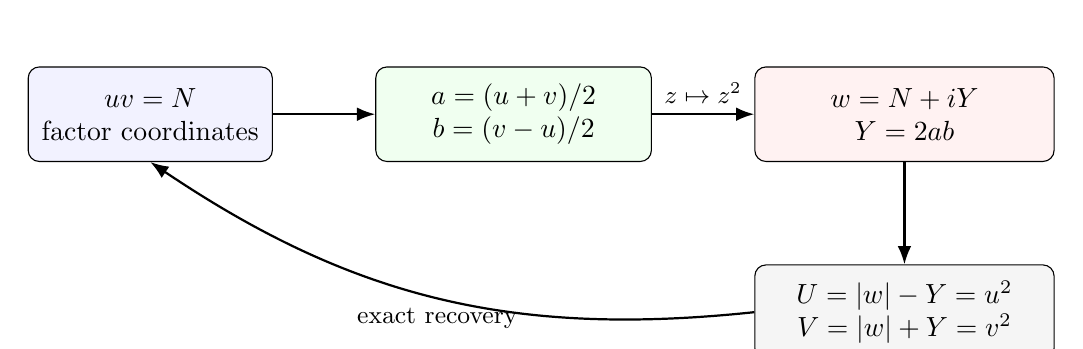
\begin{tikzpicture}[>=Latex,node distance=13mm]
  \node[draw,rounded corners,fill=blue!5,align=center,minimum width=31mm,minimum height=12mm] (factor) {$uv=N$\\factor coordinates};
  \node[draw,rounded corners,fill=green!6,align=center,minimum width=35mm,minimum height=12mm,right=of factor] (fermat) {$a=(u+v)/2$\\$b=(v-u)/2$};
  \node[draw,rounded corners,fill=red!5,align=center,minimum width=38mm,minimum height=12mm,right=of fermat] (square) {$w=N+iY$\\$Y=2ab$};
  \node[draw,rounded corners,fill=gray!8,align=center,minimum width=38mm,minimum height=12mm,below=of square] (null) {$U=|w|-Y=u^2$\\$V=|w|+Y=v^2$};
  \draw[->,thick] (factor) -- (fermat);
  \draw[->,thick] (fermat) -- node[above,font=\small] {$z\mapsto z^2$} (square);
  \draw[->,thick] (square) -- (null);
  \draw[->,thick,bend left=20] (null.west) to node[below,font=\small] {exact recovery} (factor.south);
\end{tikzpicture}
\caption{Equivalent coordinate systems on a complete factor fibre.  The squared coordinates retain the factor pair exactly.}
\label{fig:coordinate-map}
\end{figure}

%======================================================================
\section{The canonical M\"obius geometry}
\label{sec:canonical-cloud}
%======================================================================

\begin{motivation}
The M\"obius decomposition needs one reproducible point per squarefree source.  Choosing the largest prime factor supplies that point and gives a signed height that can be followed across cutoffs.
\end{motivation}

The smooth--transport decomposition does not use every point on each factor fibre.  It selects one canonical point per squarefree source.

For squarefree $m>1$, define
\begin{equation}
 q_m:=\Pplus(m),
 \qquad
 c_m:=\frac{m}{q_m}.
 \label{eq:canonical-cq}
\end{equation}
Unlike the ordered factor pair in \cref{sec:full-fibre}, the canonical pair is not reordered.  The cofactor $c_m$ may exceed $q_m$.  For example,
\[
 m=30,
 \qquad
 q_m=5,
 \qquad
 c_m=6.
\]
Therefore define the signed Fermat coordinate
\begin{equation}
 a_m:=\frac{c_m+q_m}{2},
 \qquad
 b_m:=\frac{q_m-c_m}{2}\in\frac12\Z,
 \label{eq:signed-Fermat}
\end{equation}
and the canonical squared point
\begin{equation}
 w_m:=(a_m+ib_m)^2
 =m+iY_m,
 \label{eq:canonical-w}
\end{equation}
where
\begin{equation}
 \boxed{Y_m=2a_mb_m=\frac{q_m^2-c_m^2}{2}.}
 \label{eq:signed-Y}
\end{equation}
The sign of $Y_m$ records the order of the canonical factors:
\begin{equation}
 Y_m>0\iff c_m<q_m,
 \qquad
 Y_m<0\iff c_m>q_m.
 \label{eq:Y-sign}
\end{equation}

\subsection{Parameterization by cofactors and primes}

Every squarefree $m>1$ has a unique representation
\begin{equation}
 m=cq,
 \label{eq:cq-general}
\end{equation}
where
\begin{equation}
 \mu(c)\ne0,
 \qquad
 q\text{ is prime},
 \qquad
 q>\Pplus(c).
 \label{eq:canonical-admissibility}
\end{equation}
Conversely, every pair satisfying \cref{eq:canonical-admissibility} produces a squarefree integer $m=cq$ with largest prime factor $q$.  Moreover,
\begin{equation}
 \mu(cq)=-\mu(c).
 \label{eq:canonical-sign}
\end{equation}

Define the canonical index set
\begin{equation}
 \mathscr C
 :=
 \left\{
 (c,q):
 \mu(c)\ne0,
 \ q\text{ prime},
 \ q>\Pplus(c)
 \right\}.
 \label{eq:canonical-index}
\end{equation}
The squared point cloud is
\begin{equation}
 \mathscr W
 :=
 \left\{
 cq+i\frac{q^2-c^2}{2}:(c,q)\in\mathscr C
 \right\}.
 \label{eq:canonical-cloud}
\end{equation}
The signed point measure is
\begin{equation}
 \nu
 :=
 \delta_1
 -
 \sum_{(c,q)\in\mathscr C}
 \mu(c)\,
 \delta_{\,cq+i(q^2-c^2)/2}.
 \label{eq:signed-measure}
\end{equation}
The atom at $1$ records $\mu(1)=1$.

\begin{example}[A point below the real axis]
For $m=30$, the canonical pair is $(c,q)=(6,5)$, so
\[
 a=\frac{11}{2},
 \qquad
 b=-\frac12,
 \qquad
 w_{30}=30-\frac{11}{2}i.
\]
This point enters a square prefix only after the cutoff already exceeds $q=5$, so it is smooth immediately and never occupies the transport channel.
\end{example}

%======================================================================
\section{Four equivalent coordinate systems}
\label{sec:coordinates}
%======================================================================

\begin{motivation}
Different calculations become simple in different coordinates.  The point is not to multiply notation, but to move between product, factor-gap, norm, and null coordinates without losing information.
\end{motivation}

Let
\begin{equation}
 w=x+iy
 =cq+i\frac{q^2-c^2}{2},
 \qquad
 \rho:=|w|=\sqrt{x^2+y^2}.
 \label{eq:w-rho}
\end{equation}
Then
\begin{equation}
 \rho=\frac{c^2+q^2}{2}.
 \label{eq:rho-cq}
\end{equation}
The most useful coordinate charts are collected in \cref{tab:coordinates}.

\begin{table}[htbp]
\centering
\caption{Equivalent coordinates for a canonical squared factor point.}
\label{tab:coordinates}
\renewcommand{\arraystretch}{1.35}
\begin{tabular}{>{\raggedright\arraybackslash}p{0.21\textwidth} >{\raggedright\arraybackslash}p{0.31\textwidth} >{\raggedright\arraybackslash}p{0.34\textwidth}}
\toprule
Coordinate system & Definition & Exact inverse information\\
\midrule
Factor coordinates & $(c,q)$ & $m=cq$, $q=\Pplus(m)$\\
Fermat coordinates & $a=(c+q)/2$, $b=(q-c)/2$ & $c=a-b$, $q=a+b$\\
Squared Cartesian & $x=cq$, $y=(q^2-c^2)/2$ & $w=x+iy=(a+ib)^2$\\
Radial-null & $U=\rho-y$, $V=\rho+y$ & $U=c^2$, $V=q^2$, $x^2=UV$\\
Square-root & $a^2=(\rho+x)/2$, $b^2=(\rho-x)/2$ & sign of $b$ is sign of $y$\\
\bottomrule
\end{tabular}
\end{table}

The central identities are
\begin{equation}
 \boxed{
 U:=\rho-y=c^2,
 \qquad
 V:=\rho+y=q^2.
 }
 \label{eq:UV}
\end{equation}
Consequently,
\begin{equation}
 x=\sqrt{UV}=cq,
 \qquad
 y=\frac{V-U}{2}.
 \label{eq:xy-UV}
\end{equation}

These null coordinates linearize the arithmetic cutoffs.  They also make the meaning of $2ab$ exact:
\begin{equation}
 \boxed{Y=2ab=\frac{V-U}{2},}
 \label{eq:Y-null}
\end{equation}
so the imaginary coordinate is half the separation between the squared canonical factors.

%======================================================================
\section{Fixed-cofactor parabolas}
\label{sec:cofactor-curves}
%======================================================================

\begin{motivation}
Once the cofactor is fixed, the canonical points are no longer an unstructured cloud.  They lie on explicit curves, which lets arithmetic transitions be read geometrically.
\end{motivation}

Fix a positive cofactor $c$ and let $q$ vary.  In squared Cartesian coordinates,
\begin{equation}
 x=cq,
 \qquad
 y=\frac{q^2-c^2}{2}.
 \label{eq:curve-param}
\end{equation}
Eliminating $q=x/c$ gives the cofactor parabola
\begin{equation}
 \boxed{
 \gamma_c(x)
 =\frac{x^2-c^4}{2c^2}.
 }
 \label{eq:gamma-c}
\end{equation}
The canonical point cloud is not the filled region between envelopes.  It is the arithmetic sampling
\begin{equation}
 x=cq,
 \qquad
 q\text{ prime},
 \qquad
 q>\Pplus(c),
 \label{eq:curve-sampling}
\end{equation}
on the family \cref{eq:gamma-c}.

The curve crosses the real axis at
\begin{equation}
 x=c^2.
 \label{eq:curve-axis-cross}
\end{equation}
Points to the right have $q>c$ and positive ordinate; points to the left have $q<c$ and negative ordinate.

The $c=1$ curve is
\begin{equation}
 \gamma_1(x)=\frac{x^2-1}{2}.
 \label{eq:prime-curve}
\end{equation}
Its arithmetic samples are exactly the prime points, since $m=1\cdot q=q$.  It is the outer positive envelope of the complete canonical cloud.  The curve
\begin{equation}
 \gamma_3(x)=\frac{x^2-81}{18}
 \label{eq:three-curve}
\end{equation}
is the first nontrivial odd-cofactor envelope used in semiprime search.

\begin{figure}[htbp]
\centering
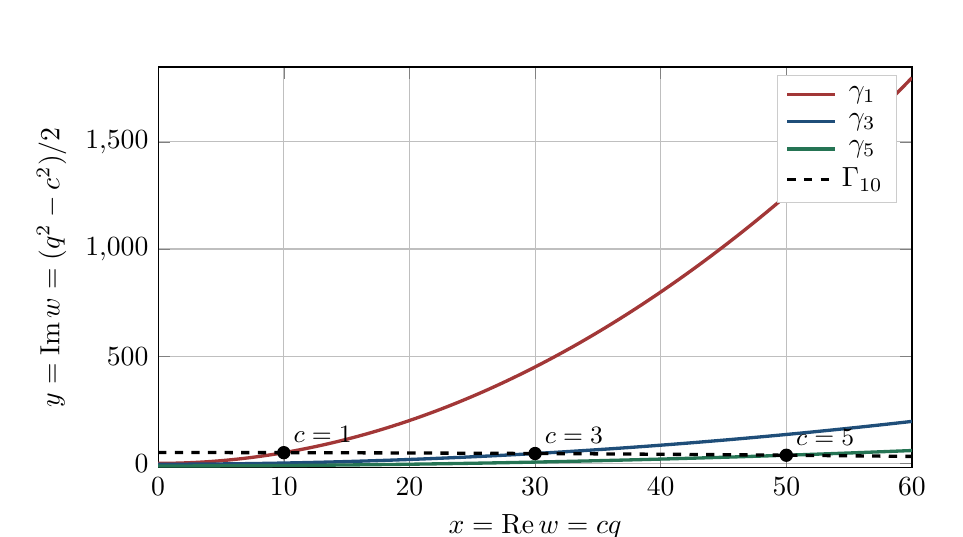
\begin{tikzpicture}
\begin{axis}[
  width=0.92\textwidth,
  height=0.55\textwidth,
  xmin=0,xmax=60,
  ymin=-20,ymax=1850,
  xlabel={$x=\Repart w=cq$},
  ylabel={$y=\Impart w=(q^2-c^2)/2$},
  grid=major,
  legend style={at={(0.98,0.98)},anchor=north east,fill=white,draw=gray!40},
  samples=240,
  domain=0:60,
  clip=true
]
  \addplot[very thick,ovvored] {(x^2-1)/2};
  \addlegendentry{$\gamma_1$}
  \addplot[very thick,ovvoblue] {(x^2-81)/18};
  \addlegendentry{$\gamma_3$}
  \addplot[very thick,ovvogreen] {(x^2-625)/50};
  \addlegendentry{$\gamma_5$}
  \addplot[very thick,black,dashed] {(10000-x^2)/200};
  \addlegendentry{$\Gamma_{10}$}
  \addplot[only marks,mark=*,mark size=2.2pt,black] coordinates {(10,49.5) (30,45.5) (50,37.5)};
  \node[anchor=south west,font=\small] at (axis cs:10,49.5) {$c=1$};
  \node[anchor=south west,font=\small] at (axis cs:30,45.5) {$c=3$};
  \node[anchor=south west,font=\small] at (axis cs:50,37.5) {$c=5$};
\end{axis}
\end{tikzpicture}
\caption{Cofactor parabolas $\gamma_c$ and the moving cutoff parabola $\Gamma_R$ for $R=10$.  Each $\gamma_c$ meets $\Gamma_R$ at $x=cR$.  Actual canonical points are discrete prime samples on the curves.}
\label{fig:cofactor-parabolas}
\end{figure}

%======================================================================
\section{Two moving boundaries}
\label{sec:moving-cutoff}
%======================================================================

\begin{motivation}
The decomposition changes with the cutoff.  The goal here is to represent that changing arithmetic classification as motion of two simple boundaries through one fixed point cloud.
\end{motivation}

Fix $R>0$.  The complete arithmetic prefix is
\begin{equation}
 \mathscr P_R
 :=\{w=x+iy\in\mathscr W:x<R^2\}.
 \label{eq:prefix-region}
\end{equation}
Since $V=q^2=|w|+y$, the smooth condition $q\le R$ is
\begin{equation}
 |w|+y\le R^2.
 \label{eq:smooth-radial}
\end{equation}
Define
\begin{align}
 \mathscr A_R
 &:={\{w\in\mathscr P_R:|w|+\Impart w\le R^2\}},
 \label{eq:A-region}\\
 \mathscr U_R
 &:={\{w\in\mathscr P_R:|w|+\Impart w>R^2\}}.
 \label{eq:U-region}
\end{align}
The prefix is the disjoint union
\begin{equation}
 \mathscr P_R=\mathscr A_R\,\dot\cup\,\mathscr U_R.
 \label{eq:region-partition}
\end{equation}

Solving \cref{eq:smooth-radial} on the boundary gives
\begin{equation}
 \boxed{
 \Gamma_R(x)=\frac{R^4-x^2}{2R^2}.
 }
 \label{eq:Gamma-R}
\end{equation}
Inside the prefix strip $x<R^2$, the smooth region lies below the graph and the transport region lies above it.

In null coordinates, the same regions are even simpler:
\begin{align}
 \mathscr P_R&:\quad UV<R^4,
 \label{eq:prefix-UV}\\
 \mathscr A_R&:\quad UV<R^4,\quad V\le R^2,
 \label{eq:smooth-UV}\\
 \mathscr U_R&:\quad UV<R^4,\quad V>R^2.
 \label{eq:transport-UV}
\end{align}
For a transport point, $UV<R^4<V^2$, so automatically $U<R^2$.  Thus
\begin{equation}
 \mathscr U_R:\quad U<R^2<V,
 \qquad
 UV<R^4.
 \label{eq:transport-null-clean}
\end{equation}
This is exactly $c<R<q$.

\subsection{Intersection with every cofactor curve}

\begin{proposition}[Intersection factorization]
\label{prop:intersection-factorization}
For $c,R>0$,
\begin{equation}
 \gamma_c(x)-\Gamma_R(x)
 =
 \frac{(R^2+c^2)(x^2-c^2R^2)}{2c^2R^2}.
 \label{eq:curve-gap}
\end{equation}
Consequently,
\begin{equation}
 \gamma_c(x)=\Gamma_R(x)
 \iff x=cR.
 \label{eq:curve-intersection}
\end{equation}
At the arithmetic point $x=cq$,
\begin{equation}
 \gamma_c(cq)-\Gamma_R(cq)
 =
 \frac{(R^2+c^2)(q^2-R^2)}{2R^2}.
 \label{eq:point-gap}
\end{equation}
\end{proposition}

The sign is therefore exact:
\begin{align}
 q<R&\iff w_{c,q}\text{ lies below }\Gamma_R,
 \label{eq:below}\\
 q>R&\iff w_{c,q}\text{ lies above }\Gamma_R.
 \label{eq:above}
\end{align}

\begin{proposition}[Orthogonal crossing]
\label{prop:orthogonal-crossing}
At the intersection $x=cR$,
\begin{equation}
 \gamma_c'(cR)=\frac{R}{c},
 \qquad
 \Gamma_R'(cR)=-\frac{c}{R},
 \label{eq:orthogonal-slopes}
\end{equation}
so
\begin{equation}
 \gamma_c'(cR)\Gamma_R'(cR)=-1.
 \label{eq:orthogonal-product}
\end{equation}
Hence each cofactor curve meets the moving cutoff orthogonally.
\end{proposition}

The transition is therefore transverse, never tangent.  A canonical point cannot remain trapped in a thin boundary layer as the cutoff passes its largest prime.

%======================================================================
\section{The moving-region interpretation of $A-T$}
\label{sec:moving-region-AT}
%======================================================================

\begin{motivation}
This section translates the algebraic identity $A-T$ into a geometric partition.  It is the bridge between the original Mertens sum and the later kernel formulation.
\end{motivation}

Using the signed measure \cref{eq:signed-measure}, define
\begin{equation}
 \mathcal A(R):=\nu(\mathscr A_R),
 \qquad
 \mathcal U(R):=\nu(\mathscr U_R).
 \label{eq:AU-measures}
\end{equation}
At $R=R_n$,
\begin{equation}
 \mathcal A(R_n)=A_n,
 \qquad
 \mathcal U(R_n)=-T_n.
 \label{eq:AU-AT}
\end{equation}
Indeed, the transport points satisfy $c<R_n<q$ and carry signed point mass
\[
 \mu(cq)=-\mu(c).
\]
Therefore
\begin{equation}
 \boxed{
 S_n
 =\nu(\mathscr P_{R_n})
 =\mathcal A(R_n)+\mathcal U(R_n)
 =A_n-T_n.
 }
 \label{eq:geometric-AT}
\end{equation}

Equivalently, define projectors
\begin{align}
 P_R(w)&:=\1_{\{\Repart w<R^2\}},
 \label{eq:P-projector}\\
 Q_R(w)&:=\1_{\{|w|+\Impart w\le R^2\}}.
 \label{eq:Q-projector}
\end{align}
Then
\begin{align}
 \mathcal A(R)&=\int P_RQ_R\,d\nu,
 \label{eq:A-projector}\\
 \mathcal U(R)&=\int P_R(1-Q_R)\,d\nu,
 \label{eq:U-projector}\\
 S(R)&=\int P_R\,d\nu.
 \label{eq:S-projector}
\end{align}
The identity is the pointwise partition
\begin{equation}
 P_R=P_RQ_R+P_R(1-Q_R).
 \label{eq:projector-partition}
\end{equation}

%======================================================================
\section{Entry, transition, and telescoping}
\label{sec:telescoping}
%======================================================================

\begin{motivation}
A source contributes at different times for different reasons.  Separating entry from transition shows which changes are genuine new data and which are internal transfers that cancel.
\end{motivation}

For a canonical source $m=cq$, define its first square-prefix index
\begin{equation}
 e(m):=\lfloor\sqrt m\rfloor.
 \label{eq:entry-index}
\end{equation}
This is the least $n$ such that $m<R_n^2$.  Define the smoothness-transition index
\begin{equation}
 h(m):=q-1.
 \label{eq:transition-index}
\end{equation}
This is the least $n$ such that $q\le R_n$.

The transport lifetime is
\begin{equation}
 L(m):=(h(m)-e(m))_+.
 \label{eq:lifetime}
\end{equation}
There are two cases:

\begin{enumerate}[leftmargin=1.7em,itemsep=0.3em]
\item If $q>\sqrt m$, equivalently $q>c$ and $Y>0$, then the point enters above the moving parabola and occupies transport for the discrete interval
\[
 e(m)\le n<h(m).
\]
\item If $q\le\sqrt m$, equivalently $q\le c$ and $Y\le0$, then $h(m)\le e(m)$ and the point enters already smooth.  Its transport interval is empty.
\end{enumerate}

Define the pointwise indicators
\begin{align}
 p_n(m)&:=\1_{\{e(m)\le n\}},
 \label{eq:p-indicator}\\
 u_n(m)&:=\1_{\{e(m)\le n<h(m)\}},
 \label{eq:u-indicator}\\
 a_n(m)&:=\1_{\{e(m)\le n,\ h(m)\le n\}}.
 \label{eq:a-indicator}
\end{align}
Then
\begin{equation}
 \boxed{p_n(m)=u_n(m)+a_n(m).}
 \label{eq:temporal-partition}
\end{equation}

\subsection{Why the crossing cancels}

Let $E_n^A$ be the signed mass entering the new vertical strip already below the moving parabola, let $E_n^U$ be the signed mass entering above it, and let $C_n$ be the signed mass crossed by the moving parabola between $R_{n-1}$ and $R_n$.  Then
\begin{align}
 \mathcal A(R_n)-\mathcal A(R_{n-1})
 &=E_n^A+C_n,
 \label{eq:Delta-A}\\
 \mathcal U(R_n)-\mathcal U(R_{n-1})
 &=E_n^U-C_n.
 \label{eq:Delta-U}
\end{align}
Therefore
\begin{equation}
 \boxed{
 S_n-S_{n-1}
 =E_n^A+E_n^U
 =\sum_{m\in B_n}\mu(m).
 }
 \label{eq:Delta-S}
\end{equation}
The entire crossing mass cancels.

\begin{figure}[htbp]
\centering
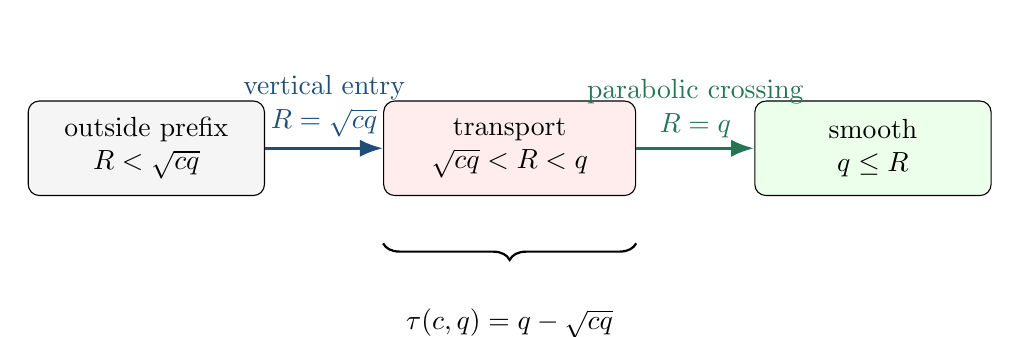
\begin{tikzpicture}[>=Latex,node distance=15mm]
  \node[draw,rounded corners,fill=gray!8,minimum width=30mm,minimum height=12mm,align=center] (out) {outside prefix\\$R<\sqrt{cq}$};
  \node[draw,rounded corners,fill=red!7,minimum width=32mm,minimum height=12mm,align=center,right=of out] (trans) {transport\\$\sqrt{cq}<R<q$};
  \node[draw,rounded corners,fill=green!8,minimum width=30mm,minimum height=12mm,align=center,right=of trans] (smooth) {smooth\\$q\le R$};
  \draw[->,very thick,ovvoblue] (out) -- node[above,align=center] {vertical entry\\$R=\sqrt{cq}$} (trans);
  \draw[->,very thick,ovvogreen] (trans) -- node[above,align=center] {parabolic crossing\\$R=q$} (smooth);
  \draw[decorate,decoration={brace,amplitude=6pt,mirror},thick] ($(trans.south west)+(0,-6mm)$) -- ($(trans.south east)+(0,-6mm)$) node[midway,below=7mm] {$\tau(c,q)=q-\sqrt{cq}$};
\end{tikzpicture}
\caption{The exact state path of a positive-height canonical point.  The second transition only reallocates signed mass between $-T$ and $A$, so it cancels from the residual increment.}
\label{fig:state-path}
\end{figure}

This is the telescopic nature of the squared coordinate: the point's imaginary height determines when the moving parabola reaches it, while the crossing itself contributes zero to the increment of the total prefix mass.

%======================================================================
\section{Why $2ab$ measures both height and lifetime}
\label{sec:lifetime-law}
%======================================================================

\begin{motivation}
The same imaginary coordinate that measures factor imbalance also measures how long a source remains in transport.  This is the key space--time link in the construction.
\end{motivation}

Define the signed continuous delay
\begin{equation}
 \tau(c,q):=q-\sqrt{cq}.
 \label{eq:tau}
\end{equation}
It is positive exactly for transport-capable points, zero at $c=q$, and negative for points that enter already smooth.

Put
\begin{equation}
 r:=\frac cq.
 \label{eq:r-ratio}
\end{equation}
Then
\begin{equation}
 Y=\frac{q^2}{2}(1-r^2)
 \label{eq:Y-r}
\end{equation}
and
\begin{equation}
 \tau=q(1-\sqrt r).
 \label{eq:tau-r}
\end{equation}
Since
\begin{equation}
 1-r^2=(1-\sqrt r)(1+\sqrt r)(1+r),
 \label{eq:factor-r}
\end{equation}
we obtain an exact identity.

\begin{theorem}[Exact height--lifetime identity]
\label{thm:exact-height-lifetime}
For every positive pair $(c,q)$,
\begin{equation}
 \boxed{
 Y
 =
 \frac{q\tau}{2}
 \left(1+\sqrt{\frac cq}\right)
 \left(1+\frac cq\right).
 }
 \label{eq:Y-tau-exact}
\end{equation}
Equivalently,
\begin{equation}
 \boxed{
 \tau
 =
 \frac{2Y}
 {q\left(1+\sqrt{c/q}\right)\left(1+c/q\right)}.
 }
 \label{eq:tau-Y-exact}
\end{equation}
\end{theorem}

The sign of $Y$ is therefore exactly the sign of the continuous delay.  On the transport side $0<c/q<1$, the denominator in \cref{eq:tau-Y-exact} lies between $q$ and $4q$, giving
\begin{equation}
 \frac{Y}{2q}
 \le\tau
 \le\frac{2Y}{q}.
 \label{eq:tau-bounds}
\end{equation}
Since
\begin{equation}
 L(m)=q-1-\lfloor\sqrt m\rfloor
 \le q-\sqrt m=\tau(c,q)
 \label{eq:L-tau}
\end{equation}
for transport points,
\begin{equation}
 \boxed{L(m)\le\frac{2Y_m}{q_m}.}
 \label{eq:L-Y}
\end{equation}

In squared-space coordinates, $q=\sqrt{|w|+\Impart w}$, so
\begin{equation}
 L(w)
 \le
 \frac{2(\Impart w)_+}
 {\sqrt{|w|+\Impart w}}.
 \label{eq:L-w}
\end{equation}
A point close to the real axis cannot remain in transport for many prefix steps.

%======================================================================
\section{Low-height clustering in square blocks}
\label{sec:clustering}
%======================================================================

\begin{motivation}
Low height is the part of the problem that geometry alone can control.  Here bounded factor gap becomes bounded occupancy, which yields a genuine theorem before any high-sector cancellation is assumed.
\end{motivation}

The $n$th square block becomes the vertical strip
\begin{equation}
 \mathscr B_n
 :=\{w_m:n^2\le\Repart w_m<(n+1)^2\}.
 \label{eq:complex-block}
\end{equation}
For a canonical pair $(c,q)$, define the absolute factor gap
\begin{equation}
 d:=|q-c|.
 \label{eq:absolute-gap}
\end{equation}
Then
\begin{equation}
 |Y|
 =\frac{|q^2-c^2|}{2}
 =\frac{d(q+c)}{2}.
 \label{eq:Y-absolute-gap}
\end{equation}
For a squarefree source $m>1$, one has $d\ge1$: equality $d=0$ would
force $m=c^2$.

\begin{lemma}[At most one product per positive absolute gap]
\label{lem:one-product-gap}
Fix $n\ge1$ and an integer $d\ge1$.  There is at most one unordered
positive factor pair $\{c,q\}$ with $|q-c|=d$ and
\begin{equation}
 n^2\le cq<(n+1)^2.
 \label{eq:gap-block-condition}
\end{equation}
\end{lemma}

\begin{proof}
Write the smaller factor as $r$ and the larger as $r+d$.  The product is
$f_d(r)=r(r+d)$.  If $f_d(r)\in B_n$, then
\[
 2r+d\ge2\sqrt{r(r+d)}\ge2n.
\]
Hence
\[
 f_d(r+1)-f_d(r)=2r+d+1\ge2n+1,
\]
which exceeds the integer diameter $2n$ of the block.  Thus two
distinct values of $r$ cannot both occur.
\end{proof}

\begin{theorem}[Sharpened absolute low-height clustering]
\label{thm:absolute-clustering}
For every $H\ge0$,
\begin{equation}
 \boxed{
 \#\{w_m\in\mathscr B_n:|Y_m|\le H\}
 \le
 \left\lfloor\frac{H}{n}\right\rfloor.
 }
 \label{eq:absolute-clustering}
\end{equation}
Moreover,
\begin{equation}
 \boxed{
 \#\{w_m\in\mathscr B_n:|Y_m|\le n\}=0.
 }
 \label{eq:no-height-n-points}
\end{equation}
\end{theorem}

\begin{proof}
If $cq\in B_n$, then
\[
 c+q\ge2\sqrt{cq}\ge2n.
\]
Therefore
\[
 |Y|=\frac{d(c+q)}2\ge dn.
\]
The condition $|Y|\le H$ implies
$d\le\lfloor H/n\rfloor$.  Since $d\ge1$, there are at most
$\lfloor H/n\rfloor$ possible gaps, and
\cref{lem:one-product-gap} gives at most one point for each gap.

If $|Y|\le n$, the inequalities force $d=1$ and $c+q=2n$.
But $|q-c|=1$ makes $c+q$ odd, whereas $2n$ is even.  Hence equality is
impossible and the set is empty.
\end{proof}

\subsection{Parity-refined bounds}

The factor gap has a prescribed parity:
\begin{itemize}[leftmargin=1.7em]
\item if $m$ is odd, then $c$ and $q$ are odd, so $d$ is even;
\item if $m$ is even and squarefree, then the canonical factors have
      opposite parity, so $d$ is odd.
\end{itemize}
Let
\begin{equation}
 D:=\left\lfloor\frac{H}{n}\right\rfloor.
 \label{eq:D-height}
\end{equation}
The permitted positive gaps are therefore
\[
 2,4,\ldots,2\left\lfloor\frac D2\right\rfloor
\]
for odd sources and
\[
 1,3,\ldots,2\left\lceil\frac D2\right\rceil-1
\]
for even sources.  Consequently,
\begin{align}
 \#\{w_m\in\mathscr B_n:m\text{ odd},\ |Y_m|\le H\}
 &\le
 \left\lfloor\frac{H}{2n}\right\rfloor,
 \label{eq:odd-parity-clustering}\\
 \#\{w_m\in\mathscr B_n:m\text{ even},\ |Y_m|\le H\}
 &\le
 \left\lceil\frac{1}{2}
 \left\lfloor\frac{H}{n}\right\rfloor\right\rceil.
 \label{eq:even-parity-clustering}
\end{align}
At the endpoint $H=n$, both populations are empty by
\cref{eq:no-height-n-points}.

At height $H=\Lambda n$, the scale-free bounds become
\begin{align}
 \#\{w_m\in\mathscr B_n:|Y_m|\le\Lambda n\}
 &\le\lfloor\Lambda\rfloor,
 \label{eq:constant-occupancy}\\
 \#\{m\text{ odd}:|Y_m|\le\Lambda n\}
 &\le\left\lfloor\frac{\Lambda}{2}\right\rfloor.
 \label{eq:constant-odd-occupancy}
\end{align}

\subsection{A sharper low-height space--time budget}

For negative-height points, the transport lifetime is zero.  For
positive-height points in $\mathscr B_n$, one has
$q\ge\sqrt m\ge n$, so \cref{eq:L-Y} gives
\begin{equation}
 L(m)\le\frac{2H}{n}
 \qquad(0<Y_m\le H).
 \label{eq:L-H-n}
\end{equation}
Therefore
\begin{equation}
 \boxed{
 \sum_{\substack{w_m\in\mathscr B_n\\|Y_m|\le H}}
 (1+L(m))
 \le
 \left\lfloor\frac{H}{n}\right\rfloor
 \left(1+\frac{2H}{n}\right).
 }
 \label{eq:space-time-budget}
\end{equation}
The parity-refined versions are
\begin{align}
 \sum_{\substack{w_m\in\mathscr B_n\\m\text{ odd},\ |Y_m|\le H}}
 (1+L(m))
 &\le
 \left\lfloor\frac{H}{2n}\right\rfloor
 \left(1+\frac{2H}{n}\right),
 \label{eq:odd-space-time-budget}\\
 \sum_{\substack{w_m\in\mathscr B_n\\m\text{ even},\ |Y_m|\le H}}
 (1+L(m))
 &\le
 \left\lceil\frac{1}{2}
 \left\lfloor\frac{H}{n}\right\rfloor\right\rceil
 \left(1+\frac{2H}{n}\right).
 \label{eq:even-space-time-budget}
\end{align}
At $H=\Lambda n$, all three right sides are bounded independently of
$n$.

%======================================================================
\section{Conformal expansion and the missing two powers}
\label{sec:jacobian}
%======================================================================

\begin{motivation}
The square map explains the scale but not the sign.  Its Jacobian supplies the required two powers of dilution; the later Gram analysis must still explain cancellation.
\end{motivation}

Consider the continuous map
\begin{equation}
 \Phi(c,q)
 :=
 \left(
 x(c,q),y(c,q)
 \right)
 =
 \left(
 cq,\frac{q^2-c^2}{2}
 \right).
 \label{eq:Phi}
\end{equation}
Its differential is
\begin{equation}
 D\Phi(c,q)
 =
 \begin{pmatrix}
 q & c\\
 -c & q
 \end{pmatrix}.
 \label{eq:D-Phi}
\end{equation}
The two columns are orthogonal and have equal length $\sqrt{c^2+q^2}$.  Consequently,
\begin{equation}
 D\Phi(c,q)^{\mathsf T}D\Phi(c,q)
 =(c^2+q^2)I.
 \label{eq:conformal-metric}
\end{equation}
Thus $\Phi$ is conformal: locally it rotates and expands every direction by the same factor
\begin{equation}
 \lambda(c,q)=\sqrt{c^2+q^2}.
 \label{eq:length-scale}
\end{equation}
The area Jacobian is
\begin{equation}
 \boxed{
 J(c,q)=\det D\Phi(c,q)=c^2+q^2=2|w|.
 }
 \label{eq:Jacobian}
\end{equation}
By AM--GM,
\begin{equation}
 c^2+q^2\ge2cq=2x.
 \label{eq:Jacobian-lower}
\end{equation}
Therefore, in the square strip $x\asymp n^2$,
\begin{equation}
 \lambda(c,q)\gtrsim n,
 \qquad
 J(c,q)\gtrsim n^2.
 \label{eq:square-scale-expansion}
\end{equation}

This is the two-dimensional version of the vertical spacing estimate.  Unit-scale separation in the factor plane becomes scale-$n$ separation in the squared plane, while unit factor-lattice area becomes scale-$n^2$ area.  The coherent square-prefix ceiling loses exactly two powers if the relevant kernel neighborhoods have bounded squared-space area after localization.

\begin{caution}[What the Jacobian does not prove]
The M\"obius point cloud is discrete and arithmetically restricted, and the square-prefix kernel is not Euclidean convolution.  The Jacobian therefore does not by itself prove a signed variance estimate.  It proves the exact geometric dilution scale that a valid operator argument must inherit.
\end{caution}


\subsection{Two-dimensional area versus one-dimensional cofactor curves}
\label{subsec:curve-versus-area}

The conformal Jacobian governs two-dimensional regions in the continuous
$(c,q)$ factor plane.  The arithmetic measure is not two-dimensional:
for each fixed cofactor $c$, it is supported on the one-dimensional
prime-sampled curve
\[
 q\longmapsto
 \Phi(c,q)
 =
 \left(cq,\frac{q^2-c^2}{2}\right),
 \qquad
 q\ \text{prime},\quad q>\Pplus(c).
\]
Along that curve,
\begin{equation}
 \left\lVert\frac{\partial\Phi}{\partial q}(c,q)\right\rVert
 =
 \sqrt{c^2+q^2}.
 \label{eq:curve-length-expansion}
\end{equation}
Thus one-dimensional arclength is also expanded, but the number and
arithmetic placement of samples are governed by primes rather than by
the area Jacobian.  A two-dimensional density estimate cannot be
applied directly to a single cofactor curve.

The outer curve $c=1$ makes this obstruction explicit.  Its contribution
to the $n$th complete prefix is
\begin{equation}
 S_n^{(1)}
 =
 -\pi(X_n),
 \label{eq:prime-curve-prefix}
\end{equation}
because every prime $q\le X_n$ has canonical pair $(1,q)$ and M\"obius
weight $-1$.  The prime number theorem therefore predicts
\begin{equation}
 \sum_{n\le N}|S_n^{(1)}|^2
 \sim
 \frac{N^5}{20\log^2 N},
 \label{eq:prime-curve-asymptotic}
\end{equation}
up to the usual slowly varying correction.  The prime curve by itself
is not on the cubic scale.  Cancellation between $c=1$ and the
aggregate of the curves $c\ge2$ is indispensable.

This also shows why a bound of the form
\[
 \sum_{q\le Q}e\!\left(\alpha\frac{q^2-c^2}{2}\right)
 \ll Q^{1/2+\eps}
\]
cannot hold uniformly in $\alpha$: at $\alpha=0$ the left side is
$\pi(Q)+O(1)$.  The zero and major-arc modes must be cancelled across
cofactor curves by the M\"obius weights $\mu(c)$ and the exact
smooth--transport architecture.  Oscillatory estimates are relevant
only after that coherent component has been isolated.


\subsection{Small-modulus prime resonances}
\label{subsec:exact-prime-resonances}

The coherent rational modes are more rigid than a generic major-arc heuristic suggests.

\begin{theorem}[Prime squares modulo $24$]
\label{thm:prime-square-mod24}
If $q>3$ is prime, then
\begin{equation}
 \boxed{q^2\equiv1\pmod{24}.}
 \label{eq:prime-square-mod24}
\end{equation}
\end{theorem}

\begin{proof}
The prime $q$ is odd, so $q^2\equiv1\pmod8$.  Also $3\nmid q$, so
$q\equiv\pm1\pmod3$ and $q^2\equiv1\pmod3$.  Since $8$ and $3$ are coprime,
the Chinese remainder theorem gives \cref{eq:prime-square-mod24}.
\end{proof}

\begin{corollary}[Perfect coherence on the $2$--$3$ resonance lattice]
\label{cor:perfect-prime-coherence}
Let $m\in\mathbb Z$ and put $\alpha=m/12$.  For every prime $q>3$,
\begin{equation}
 e\!\left(\alpha\frac{q^2}{2}\right)
 =e\!\left(\frac{m q^2}{24}\right)
 =e\!\left(\frac m{24}\right).
 \label{eq:perfect-prime-phase}
\end{equation}
Therefore, if $Q>3$,
\begin{equation}
 \boxed{
 \sum_{Q<q\le2Q\atop q\ {
m prime}}
 e\!\left(\alpha\frac{q^2}{2}\right)
 =e\!\left(\frac m{24}\right)
 \bigl(\pi(2Q)-\pi(Q)\bigr).
 }
 \label{eq:perfect-prime-sum}
\end{equation}
In particular, the magnitude equals the full prime count.
\end{corollary}

This exact coherence includes
\[
 \alpha\in\left\{0,\frac12,\frac13,\frac23,\frac14,\frac34,
 \frac16,\frac56\right\}.
\]
It is not a failure of the major/minor-arc philosophy.  It identifies a finite,
explicit resonant component that must be reproduced by the major-arc model and then
cancelled across cofactor curves.

\begin{proposition}[The rational quadratic phase has modulus $2r$]
\label{prop:phase-modulus-two-r}
Let $a,r,u\in\mathbb Z$ with $r\ne0$.  Then
\begin{equation}
 \frac{e\!\left(a(u+r)^2/(2r)\right)}
      {e\!\left(au^2/(2r)\right)}
 =(-1)^{ar}.
 \label{eq:phase-shift-r}
\end{equation}
Consequently $u\mapsto e(au^2/(2r))$ is always periodic modulo $2r$, but when
$ar$ is odd it is not a well-defined function of $u\bmod r$.
\end{proposition}

\begin{proof}
Expanding the square gives
\[
 \frac{a(u+r)^2-au^2}{2r}=au+\frac{ar}{2}.
\]
The integer term $au$ disappears under $e(t)=e^{2\pi i t}$, while
$e(ar/2)=(-1)^{ar}$.
\end{proof}

\begin{definition}[Corrected reduced quadratic prime factor]
\label{def:corrected-quadratic-factor}
For $r\ge1$ and $(a,r)=1$, define
\begin{align}
 G_{2r}^{\times}(a)
 &:={}
 \sum_{\substack{u\bmod 2r\\(u,2r)=1}}
 e\!\left(\frac{au^2}{2r}\right),
 \label{eq:corrected-reduced-Gauss}\\
 \gamma(a,r)
 &:={}
 \frac{G_{2r}^{\times}(a)}{\varphi(2r)}.
 \label{eq:normalized-corrected-factor}
\end{align}
\end{definition}

At $a=1,r=3$, the units modulo $6$ are $1$ and $5$, both with square $1$
modulo $6$.  Thus
\begin{equation}
 G_{6}^{\times}(1)=2e(1/6),
 \qquad
 \boxed{\gamma(1,3)=e(1/6),\quad |\gamma(1,3)|=1.}
 \label{eq:r3-corrected-factor}
\end{equation}
By contrast, the expression obtained by summing representatives modulo $3$ is
\[
 e(1/6)+e(4/6)=0.
\]
That vanishing is an artifact of using a modulus on which the phase is not
well-defined.

\begin{caution}[Cell-mask Fourier mass and prime-phase coherence are different]
\label{caution:cell-mask-vs-prime-phase}
The ideal prime-$3$ cell mask $(+1,-1,+1)$ has mean amplitude $1/3$ and mean-mode
energy $1/9$.  This is a statement in the cell-index Fourier variable.  It is not a
bound for the quadratic prime exponential sum at $\alpha=1/3$, whose corrected
rational factor has magnitude $1$ by \cref{eq:r3-corrected-factor}.  The coherent
prime-phase mode must first be represented explicitly and cancelled across the
M\"obius-weighted cofactor channels; only the complementary component is eligible
for the cell-mask contraction estimate.
\end{caution}

\begin{definition}[Dyadic squared-cofactor exponential sum]
\label{def:squared-cofactor-sum}
For dyadic $C,Q\ge1$, define
\begin{equation}
 F_{C,Q}(\alpha)
 :=
 \sum_{\substack{C<c\le2C\\\mu(c)\ne0}}
 -\mu(c)e\!\left(-\alpha\frac{c^2}{2}\right)
 \sum_{\substack{Q<q\le2Q\\q\ {\rm prime}\\q>\Pplus(c)}}
 e\!\left(\alpha\frac{q^2}{2}\right).
 \label{eq:F-CQ}
\end{equation}
\end{definition}

A concrete analytic route is a major/minor-arc decomposition for
$F_{C,Q}$, coupled to the Fourier representation of localized
squared-space kernels.  The major arcs must reproduce and cancel the
coherent cofactor-curve main terms, while the minor arcs must satisfy a
large-sieve or mean-square estimate.  This is the analytic content that
the conformal geometry identifies but does not itself prove.

%======================================================================
\section{Vertical spacing over a fixed product}
\label{sec:vertical-spacing}
%======================================================================

\begin{motivation}
The fixed-product fibre gives a direct spacing law.  These estimates prevent low-height points from accumulating too densely above one square block.
\end{motivation}

Fix $m>0$ and parameterize the full factor hyperbola by signed $b\in\R$:
\begin{equation}
 a=\sqrt{m+b^2},
 \qquad
 Y_m(b)=2b\sqrt{m+b^2}.
 \label{eq:Y-b}
\end{equation}
Then
\begin{equation}
 Y_m'(b)
 =2\frac{m+2b^2}{\sqrt{m+b^2}}
 \ge2\sqrt m.
 \label{eq:Y-derivative}
\end{equation}
The derivative is positive for all signed $b$, so the map is strictly increasing from the lower to the upper half-plane.

If admissible $b$ values differ by at least $h$, then
\begin{equation}
 |\Delta Y|\ge2h\sqrt m.
 \label{eq:Y-spacing}
\end{equation}
At square scale $m\asymp n^2$, vertical spacing is at least order $n$.  This agrees with the conformal scale factor in \cref{eq:square-scale-expansion}.

%======================================================================
\section{Square-prefix energy as a signed kernel}
\label{sec:variance-kernel}
%======================================================================

\begin{motivation}
Energy bounds are quadratic statements.  Rewriting the prefix variance as a kernel makes the diagonal and off-diagonal contributions visible and prepares the signed Gram formulation.
\end{motivation}

For a canonical point $w_m$, define
\begin{equation}
 p_n(w_m):=\1_{\{e(m)\le n\}}.
 \label{eq:prefix-indicator}
\end{equation}
Then
\begin{equation}
 S_n=\int p_n(w)\,d\nu(w).
 \label{eq:S-integral}
\end{equation}
For a terminal index $N$, define
\begin{equation}
 K_N(w,w')
 :=\sum_{n=1}^{N}p_n(w)p_n(w').
 \label{eq:prefix-kernel}
\end{equation}
Since each $p_n$ is a tail indicator,
\begin{equation}
 K_N(w,w')
 =
 \bigl(N-\max\{e(w),e(w')\}+1\bigr)_+.
 \label{eq:prefix-kernel-explicit}
\end{equation}
Therefore
\begin{equation}
 \boxed{
 \sum_{n=1}^{N}|S_n|^2
 =
 \iint_{\mathscr W\times\mathscr W}
 K_N(w,w')\,d\nu(w)d\nu(w').
 }
 \label{eq:variance-kernel}
\end{equation}

The channel indicators satisfy
\begin{equation}
 p_n=a_n+u_n,
 \label{eq:channel-indicator-sum}
\end{equation}
so the kernel splits exactly into smooth--smooth, transport--transport, and two cross terms.

For transport, the overlap kernel has the interval form
\begin{equation}
 K_N^{UU}(w,w')
 =
 \#\left(
 [e(w),h(w))
 \cap
 [e(w'),h(w'))
 \cap
 [1,N]
 \right).
 \label{eq:transport-overlap}
\end{equation}
Consequently,
\begin{equation}
 K_N^{UU}(w,w')
 \le\min\{L(w),L(w')\}.
 \label{eq:transport-overlap-bound}
\end{equation}
The imaginary coordinate therefore controls temporal support through \cref{eq:L-w}.

%======================================================================
\section{The proved cubic bound at low height}
\label{sec:low-cubic}
%======================================================================

\begin{motivation}
This is the closed part of the analytic argument: the low-height sector already obeys the cubic scale for geometric reasons.
\end{motivation}

Fix $\Lambda>0$.  Assign each source $m$ to its entry block
\begin{equation}
 j=e(m)=\lfloor\sqrt m\rfloor
 \label{eq:entry-block}
\end{equation}
and define the low-height block increment
\begin{equation}
 d_j^{\mathrm{low}}
 :=
 \sum_{\substack{m\in B_j\\|Y_m|\le\Lambda j}}
 \mu(m).
 \label{eq:low-block-increment}
\end{equation}
By \cref{eq:constant-occupancy},
\begin{equation}
 |d_j^{\mathrm{low}}|
 \le\lfloor\Lambda\rfloor.
 \label{eq:low-block-bound}
\end{equation}
Define
\begin{equation}
 S_n^{\mathrm{low}}
 :=\sum_{j\le n}d_j^{\mathrm{low}}.
 \label{eq:low-prefix}
\end{equation}
Even under complete sign coherence,
\begin{equation}
 |S_n^{\mathrm{low}}|
 \le\lfloor\Lambda\rfloor n.
 \label{eq:low-prefix-bound}
\end{equation}
Hence
\begin{equation}
 \boxed{
 \sum_{n\le N}|S_n^{\mathrm{low}}|^2
 \ll_{\Lambda}N^3.
 }
 \label{eq:low-cubic}
\end{equation}
No M\"obius cancellation is used.

Let
\begin{equation}
 S_n=S_n^{\mathrm{low}}+S_n^{\mathrm{high}}.
 \label{eq:low-high-split}
\end{equation}
Then
\begin{equation}
 \sum_{n\le N}|S_n|^2
 \le
 2\sum_{n\le N}|S_n^{\mathrm{low}}|^2
 +
 2\sum_{n\le N}|S_n^{\mathrm{high}}|^2.
 \label{eq:energy-low-high}
\end{equation}
Thus the low-height sector is already on the cubic scale.  The entire unresolved variance problem may be localized to the high-height point cloud.

%======================================================================
\section{The unresolved high-height problem}
\label{sec:high-sector}
%======================================================================

\begin{motivation}
Everything difficult is concentrated here.  The high sector cannot be controlled shell by shell; it requires cross-curve and cross-shell cancellation inside one operator estimate.
\end{motivation}

The high sector consists of canonical points satisfying
\begin{equation}
 |Y_m|>\Lambda e(m).
 \label{eq:high-sector}
\end{equation}
These points lie far from the real axis relative to their square scale,
but they remain highly structured:

\begin{enumerate}[leftmargin=1.7em,itemsep=0.3em]
\item they lie on the explicit curves $\gamma_c$;
\item their horizontal coordinates are prime samples $x=cq$ with
      $q>\Pplus(c)$;
\item their one-dimensional curve spacing is expanded by
      $\sqrt{c^2+q^2}$;
\item two-dimensional factor regions are expanded by
      $c^2+q^2$;
\item positive-height points have exact transport intervals
      $[e(m),h(m))$;
\item each curve crosses every moving cutoff exactly once and
      orthogonally.
\end{enumerate}

For each squarefree cofactor $c$, define the signed curve measure
\begin{equation}
 \nu_c
 :=
 -\mu(c)
 \sum_{\substack{q\text{ prime}\\q>\Pplus(c)}}
 \delta_{\,cq+i(q^2-c^2)/2}.
 \label{eq:nu-c}
\end{equation}
Then
\begin{equation}
 \nu=\delta_1+\sum_{c\ge1}\nu_c,
 \label{eq:nu-curve-sum}
\end{equation}
and the variance decomposes as
\begin{equation}
 \sum_{c,c'}
 \iint K_N(w,w')\,d\nu_c(w)d\nu_{c'}(w').
 \label{eq:curve-interactions}
\end{equation}

The curve $c=1$ is not a negligible boundary case.  By
\cref{eq:prime-curve-prefix,eq:prime-curve-asymptotic}, its unsigned
energy is of order $N^5/\log^2N$.  The cubic residual therefore requires
near-complete cancellation between this prime curve and the remaining
cofactor curves.  The numerical results in \cref{sec:numerics} measure
that cancellation directly.

\subsection{The kernel-weighted large-sieve target}

Fix a local prefix interval
\begin{equation}
 I=[N,N+H),
 \qquad 1\le H\le N,
 \label{eq:local-prefix-I}
\end{equation}
and dyadic ranges $C<c\le2C$, $Q<q\le2Q$.  Let
$\omega_{I,\ell}(c,q)$ be a smooth localization to the prefix interval,
the transport interval, and a high vertical shell $\ell$.  Define
\begin{equation}
 F_{C,Q,\ell}^{I}(\alpha)
 :=
 \sum_{\substack{C<c\le2C\\\mu(c)\ne0}}
 -\mu(c)e\!\left(-\alpha\frac{c^2}{2}\right)
 \sum_{\substack{Q<q\le2Q\\q\text{ prime}\\q>\Pplus(c)}}
 \omega_{I,\ell}(c,q)
 e\!\left(\alpha\frac{q^2}{2}\right).
 \label{eq:F-CQ-local}
\end{equation}
Let $\widehat K_{I,\ell}(\alpha)\ge0$ be the Fourier multiplier of the
corresponding localized positive semidefinite prefix/transport-overlap
kernel.

For parameters $R_0,\Delta\ge1$, define the major arcs
\begin{equation}
 \mathfrak M(R_0,\Delta)
 :=
 \bigcup_{1\le r\le R_0}
 \bigcup_{\substack{0\le a<r\\(a,r)=1}}
 \left\{
 \alpha\in\mathbb R/\mathbb Z:
 \left|\alpha-\frac ar\right|
 \le\frac{\Delta}{rN^2}
 \right\}.
 \label{eq:major-arcs}
\end{equation}
For $\alpha=a/r+\beta$ on such an arc, the rational quadratic phase is
periodic modulo $2r$ by \cref{prop:phase-modulus-two-r}.  The explicit
Hardy--Littlewood model must therefore replace the prime indicator in
\cref{eq:F-CQ-local} by its reduced-residue main term modulo $2r$:
\begin{align}
 \mathcal M_{C,Q,\ell}^{I}(\alpha)
 &:={}
 \sum_{\substack{C<c\le2C\\\mu(c)\ne0}}
 -\mu(c)e\!\left(-\alpha\frac{c^2}{2}\right)
 \gamma(a,r)
 \int_Q^{2Q}
 \omega_{I,\ell}(c,t)
 e\!\left(\beta\frac{t^2}{2}\right)
 \frac{dt}{\log t},
 \label{eq:major-arc-model-corrected}\\
 \gamma(a,r)
 &:={}
 \frac{1}{\varphi(2r)}
 \sum_{\substack{u\bmod 2r\\(u,2r)=1}}
 e\!\left(\frac{au^2}{2r}\right).
 \label{eq:quadratic-Gauss-prime-corrected}
\end{align}
Primes dividing $2r$ are treated as explicit exceptional terms; they are absent
whenever the prime range begins above $2R_0$.  Outside
$\mathfrak M(R_0,\Delta)$, put $\mathcal M_{C,Q,\ell}^{I}=0$.


Let $R_0=R_0(M)=M^{o(1)}$ be the major-arc denominator cutoff at packet scale $M$.
Let $P_{\mathrm{res},M}$ denote the orthogonal projection in the localized packet
Hilbert space onto the span of the corrected rational major-arc modes with
$r\le R_0(M)$, and put $P_{\mathrm{nr},M}=I-P_{\mathrm{res},M}$.  This is a
finite-dimensional projection at each scale, but it is not one fixed finite
projection for all scales.  For the compressed signed packet state $Z_M$, write
\begin{equation}
 Z_M=Z_M^{\mathrm{res}}+Z_M^{\mathrm{nr}},
 \qquad
 Z_M^{\mathrm{res}}=P_{\mathrm{res},M}Z_M,
 \qquad
 Z_M^{\mathrm{nr}}=P_{\mathrm{nr},M}Z_M.
 \label{eq:resonant-nonresonant-state}
\end{equation}
At each fixed scale,
\begin{equation}
 \boxed{
 \|Z_M\|^2=\|Z_M^{\mathrm{res}}\|^2+\|Z_M^{\mathrm{nr}}\|^2.
 }
 \label{eq:resonant-energy-split}
\end{equation}
The resonant term is controlled only after summing the corrected major-arc models
across the M\"obius-weighted cofactor ranges.  The nonresonant term is the proper
input to minor-arc and cell-mask contraction estimates.  Because
$P_{\mathrm{res},M}$ changes with $M$, scale descent can transfer mass between the
two components; this leakage must be included in the recursive state rather than
silently discarded.

\begin{conjecture}[Joint kernel-weighted Squared-Cofactor Large Sieve]
\label{conj:squared-cofactor-large-sieve}
For every $\eps>0$, there are choices
$R_0=N^{o(1)}$ and $\Delta=N^{o(1)}$ such that, uniformly for
$1\le H\le N$,
\begin{align}
 &\int_{\mathbb R/\mathbb Z}
 \left|
 \sum_{C,Q,\ell}
 \left(
 F_{C,Q,\ell}^{I}(\alpha)
 -\mathcal M_{C,Q,\ell}^{I}(\alpha)
 \right)
 \right|^2
 \widehat K_I(\alpha)\,d\alpha
 \ll_\eps HN^{2+\eps},
 \label{eq:cofactor-large-sieve-remainder}\\
 &\int_{\mathbb R/\mathbb Z}
 \left|
 \sum_{C,Q,\ell}
 \mathcal M_{C,Q,\ell}^{I}(\alpha)
 \right|^2
 \widehat K_I(\alpha)\,d\alpha
 \ll_\eps HN^{2+\eps}.
 \label{eq:cofactor-large-sieve-major}
\end{align}
The dyadic sums range only over cells meeting the high sector and the prefix
interval.  The sums over cofactor ranges, prime ranges, and height shells remain
\emph{inside} the absolute square.  Consequently all cross-curve, cross-shell, and
cross-frequency terms are retained.
\end{conjecture}

The first estimate is the joint kernel-weighted nonresonant and major-arc error
bound.  The second is the required cancellation of the corrected explicit
major-arc models across cofactor scales, including the exact $2$--$3$ resonance
lattice from \cref{cor:perfect-prime-coherence}.  Both clauses are necessary:
at zero frequency, and at several nonzero rational frequencies, the prime curve
has full coherent size.  A uniform pointwise square-root estimate is therefore
false.  Equally, the extended numerical experiment below shows that a positive
sum of separate shell energies is far too large.  The conjecture therefore places
the entire signed recombination in the norm generated by the square-prefix kernel.

For a finite shell partition $\{\mathscr H_\ell\}$ of the high sector, write
\begin{equation}
 S_n^{\mathrm{high}}=\sum_{\ell}S_n^{[\ell]},
 \qquad
 G_{\ell m}(N):=\sum_{n\le N}
 S_n^{[\ell]}\overline{S_n^{[m]}}.
 \label{eq:height-shell-Gram}
\end{equation}
Then
\begin{equation}
 \boxed{
 \sum_{n\le N}|S_n^{\mathrm{high}}|^2
 =\mathbf 1^*G(N)\mathbf 1
 =\sum_\ell G_{\ell\ell}(N)
 +2\Repart\sum_{\ell<m}G_{\ell m}(N).
 }
 \label{eq:height-shell-recombination}
\end{equation}

\begin{conjecture}[Joint high-sector signed Gram estimate]
\label{conj:high-kernel}
After removing the low-height sector controlled by \cref{eq:low-cubic}, the
full signed shell Gram form satisfies, for every $\eps>0$,
\begin{equation}
 \boxed{
 \mathbf 1^*G(N)\mathbf 1
 \ll_{\eps,\Lambda}N^{3+\eps}.
 }
 \label{eq:high-kernel-bound}
\end{equation}
No separate estimate $\sum_\ell G_{\ell\ell}(N)\ll N^{3+\eps}$ is assumed or
expected.  The two clauses of \cref{conj:squared-cofactor-large-sieve} are a
sufficient analytic route because they preserve the off-diagonal terms needed for
cross-shell and cross-curve cancellation.
\end{conjecture}

This formulation is stronger and more accurate than rewriting RH in the coordinate
$Y$.  It asks for control of one joint Gram matrix indexed simultaneously by
cofactor ranges, prime ranges, height shells, and rational phase modes.  The precise
analytic obstruction is not the size of the shell diagonals; it is the uniform
signed alignment of their off-diagonal interactions inside the actual-start packet
kernel.

%======================================================================

\section{Why the cubic scale is natural}
\label{sec:exponent-accounting}
%======================================================================

\begin{motivation}
Before asking for a proof, we check that every scale is dimensionally consistent.  This section explains why $N^3$, rather than the coherent $N^5$ ceiling, is the natural target.
\end{motivation}

The block increment
\begin{equation}
 d_n=S_n-S_{n-1}
 \label{eq:d-n}
\end{equation}
satisfies the trivial bound $|d_n|\le2n+1$.  Expanding the cumulative energy gives
\begin{equation}
 \sum_{n\le N}|S_n|^2
 =
 \sum_{j,k\le N}
 \bigl(N-\max\{j,k\}+1\bigr)d_jd_k.
 \label{eq:triangular-energy}
\end{equation}
The fully coherent ceiling is
\begin{equation}
 N^5
 =
 \underbrace{N}_{\text{prefix multiplicity}}
 \times
 \underbrace{N^2}_{\text{block pairs}}
 \times
 \underbrace{N^2}_{\text{raw pair amplitude}}.
 \label{eq:N5-accounting}
\end{equation}

The squared map provides the exact missing scale:
\begin{equation}
 J(c,q)=c^2+q^2\ge2cq\asymp n^2.
 \label{eq:two-power-J}
\end{equation}
Thus a unit area of factor combinations is diluted by $n^{-2}$ in the squared plane.  Equivalently, each coordinate direction is stretched by order $n$.  If the localized kernel respects this conformal dilution, then the effective pair amplitude becomes order one:
\begin{equation}
 N^3
 =
 \underbrace{N}_{\text{prefix multiplicity}}
 \times
 \underbrace{N^2}_{\text{block pairs}}
 \times
 \underbrace{1}_{\text{squared-space interaction}}.
 \label{eq:N3-accounting}
\end{equation}

The low-height theorem proves this reduction directly in the region $|Y|\lesssim n$.  The high-height conjecture asks for the corresponding operator statement in the remaining region.

%======================================================================
\section{The RH-equivalent local criterion}
\label{sec:local-criterion}
%======================================================================

\begin{motivation}
A global average is not enough to recover pointwise Mertens control.  The uniform translated-window estimate is the correct RH-equivalent statement because it allows the decisive choice $H=1$.
\end{motivation}

The global cubic energy is the natural benchmark, but a fully pointwise converse is obtained from a uniform local estimate.  Define
\begin{equation}
 V_{\mathrm{loc}}(N,H)
 :=\sum_{n=N}^{N+H-1}|S_n|^2.
 \label{eq:Vloc}
\end{equation}

\begin{theorem}[Uniform local square-prefix criterion]
\label{thm:local-RH}
The Riemann Hypothesis is equivalent to the statement that, for every $\eps>0$,
\begin{equation}
 V_{\mathrm{loc}}(N,H)
 \ll_\eps HN^{2+\eps}
 \qquad(1\le H\le N).
 \label{eq:local-RH}
\end{equation}
\end{theorem}

\begin{proof}
Under RH, the classical Mertens criterion gives
\[
 M(x)\ll_\delta x^{1/2+\delta}
\]
for every $\delta>0$.  Since $X_n\asymp n^2$, one has
\[
 |S_n|^2\ll_\eps n^{2+\eps},
\]
and summing $H$ consecutive terms gives \cref{eq:local-RH}.

Conversely, set $H=1$.  Then
\[
 |S_N|^2\ll_\eps N^{2+\eps},
\]
so $|S_N|\ll_\eta N^{1+\eta}$ for every $\eta>0$.  If
\[
 n^2\le x<(n+1)^2,
\]
then
\[
 |M(x)-M(n^2-1)|\le2n+1
\]
because $|\mu(m)|\le1$.  Therefore
\[
 M(x)\ll_\eta x^{1/2+\eta},
\]
which is equivalent to RH.
\end{proof}

A local version of \cref{conj:high-kernel} would therefore complete the argument without relying on a global-average converse.

%======================================================================
\section{Numerical evidence and preregistered diagnostics}
\label{sec:numerics}
%======================================================================

\begin{motivation}
The computations are designed to falsify mechanisms, not to certify RH.  Exact checks validate identities; asymptotic diagnostics identify where a proposed uniform theorem would first fail.
\end{motivation}

The computations reported here use exact integer arithmetic through
\begin{equation}
 N_{\max}=4096,
 \qquad
 X_{\max}=(4097)^2-1=16{,}785{,}408.
 \label{eq:numerical-range}
\end{equation}
A linear sieve produced
\begin{equation}
 1{,}078{,}362\ \text{primes}
 \qquad\text{and}\qquad
 10{,}204{,}280\ \text{squarefree sources }m\ge2.
 \label{eq:numerical-counts}
\end{equation}

\subsection{Deterministic exact checks}

The implementation independently constructed $S_n$, $A_n$, and $T_n$
from the source entry and transition intervals.  Over all $4096$
prefixes,
\begin{equation}
 \max_{n\le4096}|S_n-(A_n-T_n)|=0.
 \label{eq:exact-AT-numerical}
\end{equation}
Across all $10{,}204{,}280$ squarefree sources, the following violation
counts were also zero:

\begin{table}[htbp]
\centering
\caption{Exact squared-space verification through $X_{\max}$.}
\label{tab:exact-checks}
\small
\begin{tabular}{lr}
\toprule
Check & Violations\\
\midrule
$(q^2+c^2)^2=(2m)^2+(q^2-c^2)^2$ & 0\\
$c^2(q^2-c^2)=m^2-c^4$ & 0\\
height--lifetime inequality & 0\\
prefix identity $S_n=A_n-T_n$ & 0\\
\bottomrule
\end{tabular}
\end{table}


\subsection{Small-modulus prime-phase regression test}
\label{subsec:numerical-prime-resonance}

For the toy interval $2000<q\le4000$, there are exactly
\begin{equation}
 \pi(4000)-\pi(2000)=247
 \label{eq:toy-prime-count}
\end{equation}
primes.  Every one satisfies $q^2\equiv1\pmod{24}$.  Hence, for
$\alpha=m/12$,
\begin{equation}
 S_{\mathrm{prime}}(\alpha)
 :=\sum_{2000<q\le4000\atop q\ {
m prime}}
 e\!\left(\alpha\frac{q^2}{2}\right)
 =247e(m/24),
 \label{eq:toy-prime-resonance}
\end{equation}
and therefore $|S_{\mathrm{prime}}(\alpha)|=247$ exactly.

\begin{table}[htbp]
\centering
\caption{Exact prime-phase coherence on the tested $2$--$3$ resonance lattice.}
\label{tab:toy-prime-resonance}
\small
\begin{tabular}{ccc}
\toprule
$\alpha$ & common phase & $|S_{\mathrm{prime}}(\alpha)|$\\
\midrule
$0$ & $1$ & $247$\\
$1/2$ & $e(1/4)$ & $247$\\
$1/3$ & $e(1/6)$ & $247$\\
$2/3$ & $e(1/3)$ & $247$\\
$1/4$ & $e(1/8)$ & $247$\\
$3/4$ & $e(3/8)$ & $247$\\
$1/6$ & $e(1/12)$ & $247$\\
$5/6$ & $e(5/12)$ & $247$\\
\bottomrule
\end{tabular}
\end{table}

The old modulus-$r$ expression fails the regression test at $a=1,r=3$:
\begin{equation}
 \sum_{u\bmod3\atop(u,3)=1}e(u^2/6)=e(1/6)+e(4/6)=0.
 \label{eq:old-r3-regression-failure}
\end{equation}
The corrected units-modulo-$6$ factor is
\begin{equation}
 \frac1{\varphi(6)}
 \sum_{u\bmod6\atop(u,6)=1}e(u^2/6)
 =e(1/6),
 \label{eq:correct-r3-regression}
\end{equation}
with unit magnitude.

The elevated value at $\alpha=1/20$ is also arithmetic rather than a numerical
artifact.  For primes $q>5$, $q^2\equiv1$ or $9\pmod{40}$.  In this interval the
class counts are $123$ and $124$, respectively, so
\begin{equation}
 \left|123e(1/40)+124e(9/40)\right|
 =199.828062\ldots.
 \label{eq:one-twentieth-secondary-resonance}
\end{equation}
This illustrates why the complete reduced-square distribution modulo $2r$, not only
the denominator $r$, belongs in the rational major-arc model.

\subsection{Smooth--transport matching}

\begin{table}[htbp]
\centering
\caption{Exact cumulative prefix energies.  Every entry is computed
from all prefixes $1\le n\le N$.}
\label{tab:prefix-energy-numerical}
\scriptsize
\setlength{\tabcolsep}{4.2pt}
\begin{tabular}{rccccc}
\toprule
$N$ &
$\|A\|^2/N^3$ &
$\|T\|^2/N^3$ &
$\langle A,T\rangle/N^3$ &
$\|A-T\|^2/N^3$ &
$S_N$\\
\midrule
128  & 0.490490 & 0.469682 & 0.475665 & 0.008842 & $-18$\\
256  & 1.386025 & 1.338898 & 1.356626 & 0.011671 & $4$\\
512  & 3.709722 & 3.668905 & 3.685593 & 0.007442 & $38$\\
1024 & 9.831997 & 9.807089 & 9.814616 & 0.009853 & $288$\\
2048 & 26.661079 & 26.658451 & 26.655516 & 0.008497 & $263$\\
4096 & 72.821788 & 73.064243 & 72.938028 & 0.009974 & $329$\\
\bottomrule
\end{tabular}
\end{table}

The residual remains near the cubic scale while the two component
energies increase substantially.

\subsection{The prime curve does not satisfy the cubic bound}

Let
\[
 S_n^{(1)}=-\pi(X_n)
\]
be the contribution of the curve $c=1$, and put
\[
 S_n^{(\ge2)}=S_n-S_n^{(1)}.
\]
Then
\begin{equation}
 \|S\|^2
 =
 \|S^{(1)}\|^2
 +
 \|S^{(\ge2)}\|^2
 +
 2\langle S^{(1)},S^{(\ge2)}\rangle.
 \label{eq:prime-rest-energy}
\end{equation}

\begin{table}[htbp]
\centering
\caption{Prime-curve versus remaining-curve energy decomposition.}
\label{tab:prime-curve-decomposition}
\scriptsize
\setlength{\tabcolsep}{3.2pt}
\begin{tabular}{rcccccc}
\toprule
$N$ &
$V/N^3$ &
$V_{c=1}/N^3$ &
$V_{c\ge2}/N^3$ &
$2\langle c=1,c\ge2\rangle/N^3$ &
$V/V_{c=1}$ &
correlation\\
\midrule
128  & 0.008842 & 51.225450 & 50.965559 & $-102.182168$ & $1.7260\!\times10^{-4}$ & $-0.999916714$\\
256  & 0.011671 & 146.590116 & 146.035583 & $-292.614028$ & $7.9618\!\times10^{-5}$ & $-0.999961911$\\
512  & 0.007442 & 441.694929 & 441.211486 & $-882.898974$ & $1.6848\!\times10^{-5}$ & $-0.999991721$\\
1024 & 0.009853 & 1382.291036 & 1381.948964 & $-2764.230146$ & $7.1282\!\times10^{-6}$ & $-0.999996443$\\
2048 & 0.008497 & 4450.731250 & 4450.668331 & $-8901.391084$ & $1.9091\!\times10^{-6}$ & $-0.999999045$\\
4096 & 0.009974 & 14652.537064 & 14655.994904 & $-29308.521994$ & $6.8072\!\times10^{-7}$ & $-0.999999667$\\
\bottomrule
\end{tabular}
\end{table}

At $N=4096$, the prime curve has energy more than
$1.46\times10^4N^3$, while the total residual is approximately
$9.97\times10^{-3}N^3$.  The squared norm of the total is only
$6.81\times10^{-7}$ of the prime-curve squared norm.  This is direct
numerical evidence that the central phenomenon is cancellation
\emph{between} cofactor curves, not cubic behavior of the prime curve
in isolation.


\subsection{The dyadic cofactor cascade}
\label{subsec:cofactor-cascade}

For $C\ge1$, define the partial cofactor residual
\begin{equation}
 R_C(x)
 :=
 1-\sum_{1\le c\le C}\mu(c)\Pi_c(x),
 \label{eq:R-C}
\end{equation}
and its square-prefix energy
\begin{equation}
 V_C(N)
 :=
 \sum_{n\le N}|R_C(X_n)|^2.
 \label{eq:V-C}
\end{equation}
Thus
\[
 R_1(x)=1-\pi(x),
\]
and $R_C(x)=M(x)$ once $C$ contains every canonical cofactor that can
occur below $x$.  The cascade tests how successive dyadic cofactor
ranges cancel the prime curve.

\begin{table}[htbp]
\centering
\caption{Complete dyadic cofactor cascade at $N=4096$.  The third
column is $V_C(4096)/4096^3$; the fourth is $V_C/V_1$.  The final row is
exact because the largest observed canonical cofactor is
$692{,}835<2^{20}$.}
\label{tab:cofactor-cascade}
\scriptsize
\setlength{\tabcolsep}{7pt}
\begin{tabular}{rrrr}
\toprule
$C$ & $R_C(X_{4096})$ & $V_C/N^3$ & $V_C/V_1$\\
\midrule
1 & -1,078,361 & 14652.492160 & 1.000e+00 \\
2 & -513,936 & 3318.367550 & 2.265e-01 \\
4 & -127,056 & 198.352150 & 1.354e-02 \\
8 & 86,580 & 99.704527 & 6.805e-03 \\
16 & -4,620 & 0.148513 & 1.014e-05 \\
32 & 162,415 & 344.808298 & 2.353e-02 \\
64 & 51,754 & 36.470907 & 2.489e-03 \\
128 & 75,937 & 76.897452 & 5.248e-03 \\
256 & 67,189 & 59.850472 & 4.085e-03 \\
512 & 81,166 & 84.906888 & 5.795e-03 \\
1,024 & 71,179 & 60.275193 & 4.114e-03 \\
2,048 & 43,260 & 15.704342 & 1.072e-03 \\
4,096 & 3,633 & 4.361902 & 2.977e-04 \\
8,192 & -39,326 & 14.649760 & 9.998e-04 \\
16,384 & -15,331 & 1.552681 & 1.060e-04 \\
32,768 & -2,326 & 0.051346 & 3.504e-06 \\
65,536 & 4,622 & 0.142635 & 9.735e-06 \\
131,072 & 708 & 0.011615 & 7.927e-07 \\
262,144 & 206 & 0.009590 & 6.545e-07 \\
524,288 & 332 & 0.009980 & 6.811e-07 \\
1,048,576 & 329 & 0.009974 & 6.807e-07 \\
\bottomrule
\end{tabular}
\end{table}

The cascade is strongly nonmonotone.  The first four cofactor scales
reduce the normalized energy from $14652.49$ at $C=1$ to $0.1485$ at
$C=16$, but the next dyadic block raises it to $344.81$ at $C=32$.
Subsequent blocks repeatedly destroy and recreate coherent mass before
the residual settles near the final cubic scale.  This rules out a
simple monotone ``more cofactors means more cancellation'' picture.
The analytic estimate must control a signed cascade of dyadic
cross-terms.

The machine-readable file \texttt{cofactor\_cascade.csv} reports every
dyadic $C$ for all six prefix checkpoints
$N=128,256,512,1024,2048,4096$.


\subsection{The dyadic Gram matrix and the $16<c\le32$ spike}
\label{subsec:dyadic-Gram}

Let $B_j$ denote the complete square-prefix vector contributed by the
cofactor block
\[
 2^{j-1}<c\le2^j,
\]
with $B_0=P$ for $c=1$.  The exact Gram matrix is
\begin{equation}
 G_{ij}(N):=\langle B_i,B_j\rangle_{1\le n\le N}.
 \label{eq:dyadic-Gram}
\end{equation}
The following table compares the harmonic M\"obius coefficient
\[
 a_j=\sum_{2^{j-1}<c\le2^j}\frac{\mu(c)}{c}
\]
from \cref{thm:major-rank-one} with the finite-sample regression
coefficient
\[
 \widehat\beta_j
 :=\frac{\langle P,B_j\rangle}{\|P\|^2}.
\]

\begin{table}[htbp]
\centering
\caption{Dyadic cofactor block geometry at $N=4096$.  The close
agreement of signs, the nearly unit correlations, and the Gram spectrum
below exhibit the major-arc rank-one structure.}
\label{tab:dyadic-Gram-blocks}
\scriptsize
\setlength{\tabcolsep}{4.0pt}
\begin{tabular}{lrrrrr}
\toprule
block & $a_j$ & $\widehat\beta_j$ & corr$(P,B_j)$ & $\|B_j\|^2/N^3$ & $\Delta V/N^3$\\
\midrule
$1<c\le2$   & $-0.500000$ & $-0.524110$ & $-0.999999$ & 4024.9308 & $-11334.1246$\\
$2<c\le4$   & $-0.333333$ & $-0.359551$ & $-0.999997$ & 1894.2410 & $-3120.0154$\\
$4<c\le8$   & $-0.176190$ & $-0.198795$ & $-0.999993$ & 579.0658 & $-98.6476$\\
$8<c\le16$  & $ 0.070263$ & $ 0.085079$ & $ 0.999979$ & 106.0651 & $-99.5560$\\
$16<c\le32$ & $-0.123472$ & $-0.155995$ & $-0.999970$ & 356.5833 & $ 344.6598$\\
$32<c\le64$ & $ 0.078716$ & $ 0.103523$ & $ 0.999952$ & 157.0458 & $-308.3374$\\
\bottomrule
\end{tabular}
\end{table}

For the block $B_{16,32}$ one finds
\begin{align}
 \frac{\|B_{16,32}\|^2}{N^3}&=356.583335,\\
 \frac{\langle P,B_{16,32}\rangle}{N^3}&=-2285.725157,\\
 \operatorname{corr}(P,B_{16,32})&=-0.999970.
 \label{eq:block-16-32-prime}
\end{align}
Thus the proposed balance
$\langle P,B_{16,32}\rangle\approx-\frac12\|B_{16,32}\|^2$
is not what occurs.  Instead,
\begin{equation}
 \boxed{
 \langle P,B_{16,32}\rangle
 =-6.410073\,\|B_{16,32}\|^2
 \quad\text{at }N=4096.
 }
 \label{eq:block-16-32-ratio}
\end{equation}
The block is almost a negative scalar multiple of the prime curve, as
predicted by the rank-one theorem.

The cascade spike has a different cause.  Let $R_{16}$ be the cumulative
residual after the blocks through $c\le16$.  Then
\begin{equation}
 \frac{\langle R_{16},B_{16,32}\rangle}{N^3}
 =-5.961775,
 \label{eq:R16-block-inner}
\end{equation}
so
\begin{align}
 \frac{V_{32}-V_{16}}{N^3}
 &=\frac{\|B_{16,32}\|^2
 +2\langle R_{16},B_{16,32}\rangle}{N^3}\\
 &=356.583335-11.923550\\
 &=344.659785.
 \label{eq:block-spike-identity}
\end{align}
By $C=16$, the prime-like coherent mode has already been almost
annihilated.  The block $16<c\le32$ therefore reintroduces that mode
rather than cancelling it.  The next block $32<c\le64$ has
\[
 \frac{\langle R_{32},B_{32,64}\rangle}{N^3}=-232.691603
\]
and lowers the energy by $308.337391N^3$, repairing most of the spike.

The Gram matrix itself is nearly rank one.  For the six blocks through
$c\le32$, its largest eigenvalue contains
\begin{equation}
 0.999998101
 \label{eq:Gram-top-share-32}
\end{equation}
of the trace and
$\lambda_2/\lambda_1=1.8926\times10^{-6}$.  Through $c\le64$, the
corresponding values are $0.999997519$ and
$2.4696\times10^{-6}$.  Restricting to the high sector
$|Y|>16n$ changes these figures only to $0.999998118$ and
$1.8753\times10^{-6}$ through $c\le32$.  The observed rank-one mode is
therefore a high-sector phenomenon, not an artifact of the already
controlled low-height points.


\subsection{Independent extension through $N=2^{14}$}
\label{subsec:numerics-16384}

A separate memory-limited computation extended the exact checks and structural
diagnostics to
\begin{equation}
 N=2^{14}=16384,
 \qquad
 X_N=(16385)^2-1\approx2.68\times10^8.
 \label{eq:extended-range-16384}
\end{equation}
The larger targets $N=2^{16}$ and $2^{17}$ would require sieving past
approximately $4.3\times10^9$ and $1.7\times10^{10}$, respectively, and were not
attempted in the available memory.  No values at those scales are claimed.

The independently constructed smooth, transport, and residual values agree
exactly at every tested checkpoint.  At the terminal checkpoint,
\begin{equation}
 \boxed{
 A_{16384}=-851896,
 \qquad
 T_{16384}=-850299,
 \qquad
 S_{16384}=-1597=A_{16384}-T_{16384}.
 }
 \label{eq:extended-terminal-identity}
\end{equation}

For a cofactor block $C<c\le2C$ with $C\asymp N^\sigma$, define the
theorem-predicted rank-one residual
\begin{equation}
 E_C^{\mathrm{th}}
 :=B_C-\lambda_\sigma a_C P,
 \qquad
 \lambda_\sigma=\frac{2}{2-\sigma}.
 \label{eq:theorem-predicted-residual}
\end{equation}
This is distinct from the orthogonal least-squares residual
$B_C-\widehat\beta_CP$.  The following table reports the former.

\begin{table}[htbp]
\centering
\caption{Theorem-predicted rank-one residuals at $N=16384$.  Residual energy is
four to five orders of magnitude below the raw block energy throughout the tested
range.}
\label{tab:extended-rank-one-residuals}
\scriptsize
\setlength{\tabcolsep}{4.5pt}
\begin{tabular}{lrrrr}
\toprule
cofactor block & $a_C$ & $\|B_C\|^2/N^3$ & $\|E_C^{\mathrm{th}}\|^2/N^3$ & residual/raw\\
\midrule
$(1,2]$     & $-0.50000$ & 45202.3 & 0.5166 & $1.1\times10^{-5}$\\
$(2,4]$     & $-0.33333$ & 21074.3 & 2.4454 & $1.2\times10^{-4}$\\
$(4,8]$     & $-0.17619$ &  6344.8 & 1.0401 & $1.6\times10^{-4}$\\
$(8,16]$    & $+0.07026$ &  1133.5 & 0.0481 & $4.2\times10^{-5}$\\
$(16,32]$   & $-0.12347$ &  3752.6 & 0.1394 & $3.7\times10^{-5}$\\
$(32,64]$   & $+0.07872$ &  1626.2 & 0.4517 & $2.8\times10^{-4}$\\
$(64,128]$  & $-0.01655$ &    77.4 & 0.0547 & $7.1\times10^{-4}$\\
$(128,256]$ & $+0.00512$ &     8.9 & 0.0052 & $5.8\times10^{-4}$\\
$(256,512]$ & $-0.00911$ &    29.4 & 0.0058 & $2.0\times10^{-4}$\\
\bottomrule
\end{tabular}
\end{table}

The height-shell decomposition is more decisive.  With shells defined by the ratio
$|Y_m|/j$, where $j$ is the entry block, the diagonal shell energies are:

\begin{table}[htbp]
\centering
\caption{Height-shell diagonal energies at $N=16384$.  The recombined energy is
not the sum of these rows; it includes their large signed cross terms.}
\label{tab:extended-height-shells}
\small
\begin{tabular}{lr}
\toprule
shell for $|Y_m|/j$ & $\sum_n|S_n^{[\ell]}|^2/N^3$\\
\midrule
$[0,5)$       & 0.00057\\
$[5,20)$      & 0.0147\\
$[20,80)$     & 0.259\\
$[80,320)$    & 3.81\\
$[320,1280)$  & 44.7\\
$[1280,\infty)$ & 86.3\\
\midrule
signed recombination & 0.0104\\
\bottomrule
\end{tabular}
\end{table}

Using the rounded diagonal values in \cref{tab:extended-height-shells},
\begin{equation}
 \sum_\ell G_{\ell\ell}(N)/N^3\approx135.084,
 \qquad
 2\Repart\sum_{\ell<m}G_{\ell m}(N)/N^3\approx-135.074.
 \label{eq:extended-cross-shell-cancellation}
\end{equation}
Thus the high sector is not small by shell.  Its observed smallness is produced by
nearly complete cancellation of large off-diagonal shell interactions.  Any proof
that takes absolute values or sums separate shell norms before recombination destroys
the principal mechanism visible in the data.

\subsubsection{Exact and secondary reduced-square modes}

The exact congruence $q^2\equiv1\pmod{24}$ was verified on all $4459$ primes in
the tested prime sample.  Modulo $40$, the same sample occupied exactly the two
classes
\begin{equation}
 q^2\equiv1\text{ or }9\pmod{40},
 \label{eq:prime-square-mod40}
\end{equation}
with counts $2224$ and $2235$.  This is forced for primes $q>5$ by
$q^2\equiv1\pmod8$ and $q^2\equiv1$ or $4\pmod5$.

\begin{proposition}[Two reduced-square classes modulo $40$]
\label{prop:prime-square-mod40}
For every prime $q>5$,
\begin{equation}
 \boxed{q^2\equiv1\text{ or }9\pmod{40}.}
 \label{eq:prime-square-mod40-boxed}
\end{equation}
\end{proposition}

Accordingly, a conductor dividing $40$ produces a two-mode prime phase rather than
a featureless minor-arc sum.  In the tested sample,
\begin{center}
\begin{tabular}{lc}
\toprule
frequency & observed prime-sum magnitude\\
\midrule
$1/20$ & $3607$\\
$3/20$ & $1378$\\
$1/40$ & approximately $8$--$14$\\
$9/40$ & approximately $8$--$14$\\
\bottomrule
\end{tabular}
\end{center}
The same two exact phase modes can therefore interfere constructively or
destructively.  Here ``resonant'' means low-rank exact phase support, not necessarily
large amplitude.

Cumulative M\"obius-weighted cofactor phase magnitudes through the six blocks ending
at $c=64$ were
\begin{equation}
\begin{array}{c|rrrrrr}
\theta & (1,2]&(2,4]&(4,8]&(8,16]&(16,32]&(32,64]\\
\hline
1/12 & 1.0&1.6&3.4&4.4&8.0&13.9\\
1/20 & 1.0&1.8&2.5&5.2&7.3&10.7\\
1/40 & 1.0&2.0&1.8&2.2&0.38&2.8
\end{array}
\label{eq:extended-cofactor-phase-cascade}
\end{equation}
The $1/40$ row contains a substantial cancellation event at the block
$16<c\le32$, emphasizing again that the resonant main term is a signed cofactor
cascade rather than a monotone positive contribution.

\subsection{Low-height clustering and lifetime}

For fixed $\Lambda$, define
\begin{align}
 C_n(\Lambda)
 &:={\#}\{w_m\in\mathscr B_n:|Y_m|\le\Lambda n\},
 \label{eq:C-lambda}\\
 I_n(\Lambda)
 &:={\sum}_{\substack{w_m\in\mathscr B_n\\|Y_m|\le\Lambda n}}
 (1+L(m)).
 \label{eq:I-lambda}
\end{align}
The sharpened exact bounds are
\begin{align}
 C_n(\Lambda)&\le\lfloor\Lambda\rfloor,
 \label{eq:C-pass}\\
 I_n(\Lambda)&\le\lfloor\Lambda\rfloor(1+2\Lambda),
 \label{eq:I-pass}
\end{align}
with $C_n(1)=I_n(1)=0$.  The odd and even source counts are bounded by
$\lfloor\Lambda/2\rfloor$ and
$\lceil\lfloor\Lambda\rfloor/2\rceil$, respectively.

\begin{table}[htbp]
\centering
\caption{Observed low-height maxima over $128\le n\le4096$, with the
sharpened general and parity bounds.}
\label{tab:low-height-numerical}
\scriptsize
\setlength{\tabcolsep}{3.5pt}
\begin{tabular}{rcccccccc}
\toprule
$\Lambda$ &
count bound & total max &
odd bound & odd max &
even bound & even max &
incidence bound & incidence max\\
\midrule
1  & 0  & 0 & 0 & 0 & 0 & 0 & 0   & 0\\
2  & 2  & 1 & 1 & 0 & 1 & 1 & 10  & 1\\
4  & 4  & 2 & 2 & 1 & 2 & 1 & 36  & 4\\
8  & 8  & 4 & 4 & 2 & 4 & 2 & 136 & 10\\
16 & 16 & 6 & 8 & 3 & 8 & 3 & 528 & 26\\
\bottomrule
\end{tabular}
\end{table}

The zero at $\Lambda=1$ is now explained exactly by
\cref{eq:no-height-n-points}; it is not merely an empirical absence.
The observed total and parity occupancies remain substantially below
the sharpened deterministic envelopes.

\subsection{Uniform local ratios}

For a dyadic base $N$, define
\begin{equation}
 \mathfrak R(N)
 :=
 \max_{\substack{
 N\le M\le2N-H\\
 H\in\{1,2,4,\ldots,N\}
 }}
 \frac{\sum_{n=M}^{M+H-1}|S_n|^2}{HM^2}.
 \label{eq:worst-local-ratio}
\end{equation}

\begin{table}[htbp]
\centering
\caption{Worst local ratios from the exact range $n\le4096$.}
\label{tab:local-ratios}
\small
\begin{tabular}{rcccc}
\toprule
base $N$ &
$\mathfrak R(N)$ &
$\mathfrak R(N)/N^{0.10}$ &
maximizing start &
maximizing $H$\\
\midrule
128  & 0.176193 & 0.108459 & 243  & 1\\
256  & 0.145830 & 0.083757 & 309  & 1\\
512  & 0.183003 & 0.098069 & 547  & 1\\
1024 & 0.157837 & 0.078918 & 1032 & 1\\
2048 & 0.166479 & 0.077665 & 2544 & 1\\
\bottomrule
\end{tabular}
\end{table}

The fitted log--log slope of $\mathfrak R(N)$ over these five dyadic
scales is
\begin{equation}
 \widehat\theta=-0.00494746.
 \label{eq:local-slope}
\end{equation}
This range passes the preliminary scale-stability test
$\widehat\theta\le0.10$, but it is not long enough to determine the
asymptotic law.

\subsection{Further diagnostics}

The next numerical stage must resolve the complete joint Gram structure, not merely
produce additional diagonal energies.  At each dyadic scale it should report:

\begin{enumerate}[leftmargin=1.7em,itemsep=0.3em]
\item both the theorem-predicted coefficient $\lambda_\sigma a_C$ and the exact
      orthogonal coefficient $\widehat\beta_C$ for every cofactor block;
\item the full height-shell Gram matrix $G_{\ell m}$ and its spectrum;
\item cross-shell contributions grouped by cofactor and prime ranges;
\item exact reduced-square phase classes modulo $2r$ for all retained major arcs;
\item the resonant/nonresonant leakage created by replacing
      $P_{\mathrm{res},M}$ with $P_{\mathrm{res},M'}$ under scale descent;
\item the low-height and endpoint forcing vectors before and after projection;
\item the contribution of every indexed cell to the full signed quantity
      $\mathbf1^*G_M\mathbf1$.
\end{enumerate}

The preregistered pass condition is no longer that each shell or localized cell be
small.  It is that the full recombined Gram form obey a scale-uniform bound after the
explicit major-arc modes have been modeled with modulus $2r$.  A computation may
therefore pass even when individual shell diagonals grow, provided the corresponding
off-diagonal cancellation is stable and quantitatively explained.  Conversely, a
small aggregate residual without a stable cross-shell and cross-curve mechanism is
not evidence for the required uniform theorem.

%======================================================================

\section{Machine-checked formalization}
\label{sec:lean}
%======================================================================

\begin{motivation}
Formalization is used here as a mathematical audit.  It forces every index, modulus, projection, sign, and quantifier to be stated explicitly.  In particular, it exposed the difference between a global cubic average and the genuinely RH-equivalent uniform local estimate.
\end{motivation}

The accompanying Lean 4 project is available at
\[
 \texttt{https://github.com/OVVO-Financial/RH\_Lean}.
\]
It is pinned to mathlib \texttt{v4.24.0} and currently imports thirty-five theorem modules.  The source audit rejects \texttt{sorry}, \texttt{admit}, newly introduced axioms, and hidden theorem substitutes; the full library is built with warnings treated as errors.

The formal development is organized by dependency rather than by the narrative order of this paper.

\subsection{Arithmetic, phase, and geometry}

The compiled arithmetic layer includes M\"obius doubling, four-slot compression, deterministic prime-$3$ activation, the prime-square congruence modulo $24$, and the two square classes modulo $40$.  The phase layer uses the canonical modulus $2r$, proves the shift-by-$r$ sign law, defines the reduced Gauss factor over $(\mathbb Z/2r\mathbb Z)^\times$, and keeps the prime-$3$ cell-mask energy separate from the prime-$3$ quadratic resonance.

The geometry layer formalizes Fermat midpoint/half-gap coordinates, squared-complex recovery, cofactor parabolas, the $2ab$ displacement laws, conformality of the square map, and the two-sheeted square fibre with positive-branch injectivity.

\subsection{Signed Gram and residual architecture}

The Hilbert-space layer proves the exact height-shell Gram identity with every off-diagonal real inner product retained.  It defines the true orthogonal coefficient and residual, proves orthogonality and the Pythagorean identity, and keeps that projection separate from the theorem-predicted coefficient used in the number-theoretic decomposition.

Subsequent modules define the scale-dependent resonant projection, resonant/nonresonant leakage, the weighted affine Lyapunov closure, the fully indexed actual residual, exact resonant cancellation for certified M\"obius cofactor pairs, forcing estimates, and the full shell/cofactor/mode/row signed Gram recombination.  No theorem replaces the joint signed form by separate positive shell bounds.

\subsection{Certificates, actual-start identities, and localization}

The finite-range checker verifies exact integer checkpoint data and has a proved soundness theorem.  Acceptance of a certificate is deliberately separate from the mathematical realization that identifies the checked data with the analytic quantities in this paper.

The actual-start modules formalize
\[
 \operatorname{actual}(M)
 =2\operatorname{prediction}(M)+\operatorname{residual}(M)
\]
and the exact signed energy identity
\[
 \begin{aligned}
 \operatorname{actualEnergy}
 &=4\operatorname{predictionEnergy}
 +\operatorname{residualEnergy}\\
 &\qquad+\operatorname{signedPredictionResidualInteraction}.
 \end{aligned}
\]
The sharp constant-$4$ inequality is obtained only when the signed interaction explicitly absorbs the residual budget.

The corrected localization layer repeats these definitions on every interval $[N,N+H)$.  It introduces a separate local signed-interaction hypothesis, proves the exact windowed energy identity, and proves the sharp local frame inequality.  A prefix estimate beginning at zero is never used as a substitute for a translated local estimate.

\subsection{The corrected RH bridge}

The formal RH target is the manuscript's local criterion
\[
 V_{\mathrm{loc}}(N,H)\ll_\eps HN^{2+\eps},
 \qquad 1\le H\le N,
\]
not merely the global benchmark $V(N)=O(N^{3+\eps})$.  Lean proves the elementary localization step from the uniform local estimate to the pointwise bound by taking $H=1$.

The final bridge then has the schematic form
\[
 \begin{gathered}
 \text{local signed frame}
 \Longrightarrow \text{uniform local square-prefix bound}
 \Longrightarrow \text{pointwise square-prefix bound}\\
 \Longrightarrow \text{Riemann Hypothesis}.
 \end{gathered}
\]
The reverse RH-to-local implication is retained separately so that the criterion can be stated as an equivalence.

What Lean currently proves is an axiom-free conditional composition theorem: all remaining implications are ordinary typed premises, not project axioms.  The unconstructed inputs are the concrete prediction estimate giving the $HN^{2+\eps}$ scale, the identification of the formal actual-start coefficient with the square-prefix Mertens value, the two classical Mertens/RH directions, and the concrete realization, contraction, starting-configuration, and local signed-interaction instances.

This is the intended boundary.  The formalization does not claim RH; it records exactly what has been reduced to what, and prevents a global-average statement from being mistaken for the local criterion.

%======================================================================
\section{Fixed packets, small-prime channels, and uniform control}
\label{sec:fixed-packet}
%======================================================================

\begin{motivation}
The packets themselves do not change when the observation horizon grows.  Making that fixedness explicit removes a false source of operator evolution and isolates the real scale-dependent leakage.
\end{motivation}

This section isolates a logical point that is easy to obscure when one works with a
family of finite matrices indexed by the scale.  The arithmetic packets themselves do
not change as the horizon grows.  What changes is only which fixed packets are being
observed and how they are normalized.  This distinction removes a spurious source of
``operator evolution'' and places the remaining proof obligation in its sharpest form.

\subsection{A universal fixed packet system}

Retain the complete half-square grid
\[
 X_m=\left\lfloor\frac{m^2}{2}\right\rfloor
\]
and the complete block sums
\[
 \Delta_m:=M(X_{m+1})-M(X_m)
 =\sum_{X_m<n\le X_{m+1}}\mu(n).
\]
For every starting index $u$ and length $L$, define the complete packet
\begin{equation}
 \mathcal B_{u,L}:=(X_u,X_{u+L}],
 \qquad
 S_{u,L}:=\sum_{m=u}^{u+L-1}\Delta_m.
 \label{eq:fixed-packet-def}
\end{equation}
Once $u$ and $L$ are fixed, both $\mathcal B_{u,L}$ and $S_{u,L}$ are fixed forever.
Passing to a larger horizon does not alter any earlier block or packet.

\begin{proposition}[No retroactive packet deformation]
\label{prop:no-retroactive}
For every $u,L$ and every observation horizon $H\ge u+L$, the value of
$S_{u,L}$ is independent of $H$.  If a finite packet vector is enlarged by appending
additional packet coordinates, its previously existing coordinates are unchanged.
\end{proposition}

\begin{proof}
The value in \cref{eq:fixed-packet-def} is a finite sum of the already fixed block
values $\Delta_u,\ldots,\Delta_{u+L-1}$.  No later block occurs in that sum.
\end{proof}

It is therefore preferable to define one universal incidence system.  For an
arithmetic source $w$, let
\[
 \Phi_w(u,L):=\1_{\{w\in\mathcal B_{u,L}\}}.
\]
The infinite column $\Phi_w$ is fixed.  A scale-$M$ operator is merely a coordinate
restriction
\[
 P_M\Phi_w=\bigl(\Phi_w(u,M)\bigr)_{M\le u<2M}.
\]
If $A_\infty$ denotes the universal synthesis map, then
\begin{equation}
 A_M=P_MA_\infty,
 \qquad
 K_M=A_\infty^*P_M^*P_MA_\infty.
 \label{eq:universal-restriction}
\end{equation}
Thus $K_M$ changes with $M$ only because the observation projection changes.  The
arithmetic columns do not move.

For nested square prefixes the same point is even more transparent.  Let
\[
 p_n(w):=\1_{\{e(w)\le n\}}.
\]
Then the prefix kernel satisfies the exact rank-one update
\begin{equation}
 K_{N+1}=K_N+p_{N+1}\otimes p_{N+1},
 \label{eq:rank-one-prefix-update}
\end{equation}
and consequently
\begin{equation}
 V(N+1)=V(N)+|S_{N+1}|^2.
 \label{eq:variance-append}
\end{equation}
No previous term is changed.

\subsection{The role of the $2ab$ coordinate}

The fixed-packet formulation corrects the interpretation of the squared height.
The coordinate
\[
 Y=2ab=\frac{q^2-c^2}{2}
\]
does not describe how an old packet deforms when a new packet is added.  It determines
the permanent activation interval of the canonical factor point.  If
\[
 e(cq)=\lfloor\sqrt{cq}\rfloor,
 \qquad h(cq)=q-1,
\]
then
\[
 I(c,q):=\{n:e(cq)\le n\le h(cq)\}
\]
is fixed, and its incidence column is
\[
 \phi_{c,q}(n)=\1_{I(c,q)}(n).
\]
The exact continuous lifetime identity from \cref{sec:lifetime-law} may be written
\begin{equation}
 Y
 =\frac{q\tau}{2}
   \left(1+\sqrt{c/q}\right)\left(1+c/q\right),
 \qquad
 \tau=q-\sqrt{cq}.
 \label{eq:Y-fixed-lifetime}
\end{equation}
Hence $Y/q$ controls the length of a fixed incidence interval.  Differences in
$Y$ control differences among fixed columns; they do not cause retroactive changes.

For the low-frequency atoms
\[
 v_r(\theta)=\1_{[-1/N,1/N]}(\theta)e(r\theta),
\]
one has, for $|r-s|\ll N$,
\begin{equation}
 \norm{v_r-v_s}_2^2
 =\frac{8\pi^2}{3}\frac{(r-s)^2}{N^3}
 +O\!\left(\frac{(r-s)^4}{N^5}\right).
 \label{eq:packet-column-modulus}
\end{equation}
Consequently, the $2ab$ spacing controls a modulus of continuity for the fixed packet
columns.  This is the functional-analytic image of the squared-space spacing law.

\subsection{Least-prime channels}

Every squarefree integer $n>1$ has the unique small-prime representation
\[
 n=pa,
 \qquad p=P^-(n),
 \qquad P^-(a)>p,
 \qquad \mu(pa)=-\mu(a).
\]
For the fixed packet $\mathcal B_{u,M}$, define
\begin{equation}
 L_{p,M}(u)
 :=-\!\!\sum_{\substack{X_u/p<a\le X_{u+M}/p\\
                         \mu(a)\ne0,\ P^-(a)>p}}
       \mu(a).
 \label{eq:small-prime-layer-fixed}
\end{equation}
Then, coordinatewise,
\begin{equation}
 \vect S_M=\sum_p\vect L_{p,M}.
 \label{eq:small-prime-fixed-recursion}
\end{equation}
This is an identity among fixed packet vectors.  The $p=2$ channel is the exact
sign-reversed odd squarefree parent process at numerical scale $1/2$, corresponding
to block scale $M/\sqrt2$.  Every $p\ge3$ parent lies at numerical scale at most
$1/3$.

\subsection{Dyadic sign-flip cells}
\label{subsec:exact-dyadic-cells}

The prime-$2$ mechanism is stronger than a channel-level heuristic.  It compresses
the raw M\"obius sequence into an exact permanent four-slot cell before averaging,
projection, or asymptotic estimation.

\begin{theorem}[Exact dyadic sign reversal]
\label{thm:exact-dyadic-sign-reversal}
For every odd integer $a\ge1$,
\begin{equation}
 \boxed{\mu(2a)=-\mu(a).}
 \label{eq:mobius-doubling-odd}
\end{equation}
This includes nonsquarefree $a$, for which both sides vanish.
\end{theorem}

\begin{proof}
If $a$ is squarefree, then $\gcd(2,a)=1$ and multiplicativity gives
$\mu(2a)=\mu(2)\mu(a)=-\mu(a)$.  If $a$ is not squarefree, the same prime
square divides both $a$ and $2a$, so both M\"obius values are zero.
\end{proof}

Taking $a=2k+1$ and using $4\mid4k+4$ yields
\begin{equation}
 \mu(4k+2)=-\mu(2k+1),
 \qquad
 \mu(4k+4)=0.
 \label{eq:dyadic-two-identities}
\end{equation}

\begin{theorem}[Exact four-slot cell compression]
\label{thm:exact-four-slot-cell}
Define
\[
 \mathbf C_k
 :=\bigl(\mu(4k+1),\mu(4k+2),\mu(4k+3),\mu(4k+4)\bigr).
\]
Then
\begin{equation}
 \boxed{
 \mathbf C_k
 =\bigl(\mu(4k+1),-\mu(2k+1),\mu(4k+3),0\bigr).
 }
 \label{eq:exact-four-slot-cell}
\end{equation}
Its scalar compression is
\begin{equation}
 \boxed{
 C_k=\mu(4k+1)-\mu(2k+1)+\mu(4k+3).
 }
 \label{eq:compressed-cell}
\end{equation}
\end{theorem}

The pattern $(+,-,+,0)$ is therefore exact.  At the fixed-column level,
\begin{equation}
 \mu(a)\phi_a+\mu(2a)\phi_{2a}
 =\mu(a)(\phi_a-\phi_{2a}),
 \label{eq:exact-doubling-column-difference}
\end{equation}
so the common component cancels before the packet norm is formed.

\subsubsection{Universal prime-$3$ activation}

Since $4\equiv1\pmod3$, the three active slots have residues
$k+1,k+2,k$ modulo $3$.

\begin{theorem}[Prime-$3$ active-slot cycle]
\label{thm:prime-three-active-slot-cycle}
Exactly one of $4k+1,4k+2,4k+3$ is divisible by $3$.  The affected slot is
\begin{equation}
 \begin{array}{c|c}
 k\bmod3&\text{active multiple of }3\\
 \hline
 0&4k+3\\
 1&4k+2\\
 2&4k+1
 \end{array}
 \label{eq:prime-three-slot-cycle}
\end{equation}
\end{theorem}

Thus prime $2$ first creates the exact three-active-channel cell, and prime $3$
then acts on one compulsory channel in every cell.  Up to cyclic translation, the
ideal live sign mask is
\[
 m_3=(+1,-1,+1),
\]
whose normalized Fourier squared magnitudes are
\begin{equation}
 \frac19,\qquad\frac49,\qquad\frac49.
 \label{eq:p3-cell-fourier-masses}
\end{equation}
The mean-mode energy factor $1/9$ concerns the cell-index mask only.  By
\cref{caution:cell-mask-vs-prime-phase}, it does not suppress the exactly coherent
quadratic prime phase at $\alpha=1/3$.

\subsubsection{Complete-cell and half-square packet equivalence}

For a finite cell-index interval $I$,
\begin{equation}
 \boxed{
 \sum_{n\in4I+\{1,2,3,4\}}\mu(n)
 =\sum_{k\in I}C_k.
 }
 \label{eq:complete-cell-packet-identity}
\end{equation}
For an arbitrary integer interval $(A,B]$, complete cells leave only two endpoint
fragments, so
\begin{equation}
 \sum_{A<n\le B}\mu(n)
 =\sum_{k\in\mathcal K(A,B)}C_k+E(A,B),
 \qquad |E(A,B)|\le6.
 \label{eq:arbitrary-cell-packet}
\end{equation}

For the half-square grid $X_m=\lfloor m^2/2\rfloor$, each endpoint is $0$ or $2$
modulo $4$.  A fragment adjacent to an endpoint of class $2$ contains a multiple of
$4$, whose M\"obius value is zero.  Therefore the fixed packet
$\mathcal B_{u,M}=(X_u,X_{u+M}]$ satisfies
\begin{equation}
 \boxed{
 S_{u,M}
 =\sum_{k=\lceil X_u/4\rceil}^{\lfloor X_{u+M}/4\rfloor-1}
 \bigl[\mu(4k+1)-\mu(2k+1)+\mu(4k+3)\bigr]
 +E_{u,M},
 }
 \label{eq:half-square-compressed-packet}
\end{equation}
with
\begin{equation}
 \boxed{|E_{u,M}|\le3,
 \qquad
 \sum_{u=M}^{2M-1}|E_{u,M}|^2\le9M.}
 \label{eq:half-square-boundary-energy}
\end{equation}

Define
\begin{equation}
 \widetilde S_{u,M}
 :=\sum_{k=\lceil X_u/4\rceil}^{\lfloor X_{u+M}/4\rfloor-1}
 \bigl[\mu(4k+1)-\mu(2k+1)+\mu(4k+3)\bigr].
 \label{eq:compressed-packet-state}
\end{equation}
Then $S_{u,M}=\widetilde S_{u,M}+E_{u,M}$ with boundary energy $O(M)$, so the
raw and compressed packet-energy criteria are equivalent at the
$M^{3+\eps}$ scale.  The primary actual-start problem is therefore
\begin{equation}
 \boxed{
 \sum_{u=M}^{2M-1}|\widetilde S_{u,M}|^2
 \ll_\eps M^{3+\eps}.
 }
 \label{eq:compressed-master-variance}
\end{equation}
The open operator estimate acts on this already compressed signed process.

\subsection{Small-prime cell contraction versus rational resonances}

The prime-$2$ parity mask has the exact low-mode factor
\begin{equation}
 \rho_2=\frac{35+3\sqrt{65}}{70}=0.845525332\ldots.
 \label{eq:rho2-fixed}
\end{equation}
For the ideal cell mask, the prime-$3$ mean-mode energy factor is
\begin{equation}
 \rho_{3,\mathrm{cell}}=\frac19.
 \label{eq:rho3-cell-fixed}
\end{equation}
These factors can enter a global contraction budget only after the corrected rational
major-arc component has been projected out or explicitly included in the parent state.
The exact modes from \cref{cor:perfect-prime-coherence} are not leakage errors; they
are genuine coherent modes requiring cofactor cancellation.

\subsection{The signed Gram form}

Separate the fixed child-feature columns by the sign of the parent cofactor and write
\[
 Z_+=\sum_{\mu(a)=+1}\Phi_{a,M},
 \qquad
 Z_-=\sum_{\mu(a)=-1}\Phi_{a,M}.
\]
The exact signed packet state is $Z_+-Z_-$.  If
\[
 A=\norm{Z_+}^2,
 \qquad B=\norm{Z_-}^2,
 \qquad
 \cos\vartheta=\frac{\Repart\ip{Z_+}{Z_-}}{\sqrt{AB}},
\]
then
\begin{equation}
 \norm{Z_+-Z_-}^2
 =\left(\sqrt A-\sqrt B\right)^2
  +2\sqrt{AB}\left(1-\cos\vartheta\right).
 \label{eq:directional-defect-fixed}
\end{equation}
The two terms are respectively the directional mass defect and the directional
profile defect.  The required cancellation is therefore not generic orthogonality;
it is near-concordance of the two opposite-sign aggregate profiles.

Equivalently, with synthesis operators $U_M$ and $V_M$ for the two sign classes, the
joint Gram matrix is
\[
 \mathbb G_M=
 \begin{pmatrix}
  U_M^*U_M&U_M^*V_M\\
  V_M^*U_M&V_M^*V_M
 \end{pmatrix}\succeq0.
\]
A natural sufficient condition is a small pair of Schur-complement defects, together
with spectral balance of $U_M^*U_M$ and $V_M^*V_M$.  This is the operator form of
concordance saturation.

\subsection{Uniform bounds and the quantifier issue}

The fixedness of every finite packet does not by itself give the RH estimate.  The
necessary assertion is a uniform bound with one constant independent of the scale.
Define
\begin{equation}
 q_\eps(N):=\frac{V(N)}{N^{3+\eps}},
 \qquad
 Q_\eps(N):=\sup_{1\le m\le N}q_\eps(m).
 \label{eq:normalized-energy-fixed}
\end{equation}
The target is
\begin{equation}
 \boxed{\displaystyle
  \sup_{N\ge1}q_\eps(N)<\infty.}
 \label{eq:finite-uniform-bound}
\end{equation}
This is the precise sense in which the proof requires a finite bound with no growing
$N$-dependent coefficient.  It is not enough that for each fixed $N$ one may choose a
new constant $C_N$.

\begin{theorem}[Uniform closure from strict scale descent]
\label{thm:uniform-closure}
Suppose that there exist $N_0$, $0<\rho<1$, $\eta>0$, and $C_\eps<\infty$, all
independent of $N$, such that for $N\ge N_0$,
\begin{equation}
 q_\eps(N)
 \le \rho\,Q_\eps\!\left(N/\sqrt2+O(1)\right)
      +C_\eps N^{-\eta}.
 \label{eq:strict-scale-recursion}
\end{equation}
Then \cref{eq:finite-uniform-bound} holds.  In particular,
\[
 V(N)\ll_\eps N^{3+\eps}.
\]
\end{theorem}

\begin{proof}
Iterate \cref{eq:strict-scale-recursion} until the ancestral scale is at most $N_0$.
After $k\asymp\log N$ steps,
\[
 q_\eps(N)
 \le \rho^kQ_\eps(N_0)
 +C_\eps\sum_{j=0}^{k-1}
   \rho^j\left(N2^{-j/2}\right)^{-\eta}.
\]
Choose $\eta>0$ small enough that $\rho2^{\eta/2}<1$.  The geometric series is
uniformly bounded, and the first term tends to zero.  Enlarging the final constant to
cover $N<N_0$ proves the claim.
\end{proof}

The theorem shows exactly why the fixed-packet insight is useful but not circular.
It eliminates retroactive deformation and leaves only a uniform smaller-scale
comparison.  Once the coefficient $\rho$ is strictly below one, the finite uniform
bound is elementary.

\subsection{The resonant/nonresonant channel budget}

Let $P_{\mathrm{res},M}$ be the scale-dependent rational-mode projection from
\cref{eq:resonant-nonresonant-state}.  The candidate prime budget applies only to
the nonresonant diagonal action after all retained modulus-$2r$ modes have been
extracted.  Its orientation value remains
\begin{equation}
 \rho_{\mathrm{nr,cand}}
 =2^{-3/2}\rho_2
  +3^{-3/2}\rho_{3,\mathrm{cell}}
  +\rho_{\ge5,\mathrm{nr}},
 \label{eq:candidate-budget-corrected}
\end{equation}
and, conditionally on
\begin{equation}
 \rho_{\ge5,\mathrm{nr}}
 \le\sum_{p\ge5}p^{-3/2}+o(1),
 \label{eq:pge5-budget-corrected}
\end{equation}
the numerical orientation
\begin{equation}
 2^{-3/2}\rho_2
 +3^{-3/2}\frac19
 +\sum_{p\ge5}p^{-3/2}
 \approx0.624
 \label{eq:point-six-two-four-budget}
\end{equation}
leaves a margin below one.  This is not a bound for the full state, and it is not
even sufficient for the projected state unless resonant/nonresonant leakage and
additive forcing are controlled.  The facts $|\gamma(1,3)|=1$ and
$\rho_{3,\mathrm{cell}}=1/9$ remain compatible because they act in different
Fourier variables.

To expose the feedback explicitly, let
\[
 R_M=P_{\mathrm{res},M}Z_M,
 \qquad
 N_M=P_{\mathrm{nr},M}Z_M.
\]
A parent-to-child descent has the schematic form
\begin{equation}
 \begin{pmatrix}R_M\\N_M\end{pmatrix}
 =
 \begin{pmatrix}A_M&B_M\\C_M&D_M\end{pmatrix}
 \begin{pmatrix}R_{\mathrm{par}(M)}\\N_{\mathrm{par}(M)}\end{pmatrix}
 +
 \begin{pmatrix}f_M^{R}\\f_M^{N}\end{pmatrix}.
 \label{eq:resonant-block-recursion}
\end{equation}
Here $B_M$ and $C_M$ include projection leakage, while $f_M^R,f_M^N$ contain
low-height, endpoint, and completion forcing.  A bound on $D_M$ alone does not
close the argument.

\begin{conjecture}[Joint actual-start block Lyapunov contraction]
\label{conj:corrected-fixed-packet-frame}
For every $\eps>0$ there exist $\eta>0$, $0<\rho<1$, $C_\eps<\infty$, and a
positive definite scale-uniform Lyapunov form $\mathcal L$ such that, for every
actual-start compressed packet state,
\begin{equation}
 \boxed{
 \left\|
 \begin{pmatrix}A_M&B_M\\C_M&D_M\end{pmatrix}
 \right\|_{\mathcal L}
 \le\rho<1,
 }
 \label{eq:block-Lyapunov-contraction}
\end{equation}
and
\begin{equation}
 \boxed{
 \left\|\begin{pmatrix}f_M^R\\f_M^N\end{pmatrix}\right\|_{\mathcal L}^2
 \le C_\eps M^{3-\eta+\eps}.
 }
 \label{eq:block-forcing-bound}
\end{equation}
The Lyapunov energy is the full actual-start signed Gram form: sums over height
shells, cofactor ranges, prime modes, and resonant/nonresonant components remain
inside the norm.  All Fejer weights, cross-cell terms, cross-prime terms, boundary
fragments, and ancestral completion terms are retained.
\end{conjecture}

A slightly weaker sufficient alternative is a triangular theorem in which the
resonant component is bounded independently, the leakage into the nonresonant
component is summable, and the nonresonant diagonal block contracts uniformly.
Either formulation must prevent low-height or boundary forcing from being
reprojected coherently into a later resonant mode.

Combining \cref{conj:corrected-fixed-packet-frame} with
\cref{thm:uniform-closure} yields the finite normalized bound.  The corrected final
target is therefore
\begin{equation}
 \boxed{
 \begin{aligned}
 &\text{joint resonant cancellation}
 +\text{cross-shell signed Gram control}\\
 &\qquad
 +\text{nonresonant contraction}
 +\text{leakage/forcing control}.
 \end{aligned}
 }
 \label{eq:final-two-part-target}
\end{equation}

%======================================================================
\section{What is proved, formalized, and still open}
\label{sec:status}
%======================================================================

\begin{motivation}
There are three different claims to track: a result may be proved in the manuscript, formalized in Lean, or still required for the RH implication.  Combining those categories into a single word such as ``proved'' would obscure the actual state of the program.
\end{motivation}

\begin{table}[htbp]
\centering
\caption{Mathematical and formal status of the program.}
\label{tab:status}
\small
\renewcommand{\arraystretch}{1.22}
\begin{tabular}{>{\raggedright\arraybackslash}p{0.46\textwidth}
                >{\raggedright\arraybackslash}p{0.20\textwidth}
                >{\raggedright\arraybackslash}p{0.22\textwidth}}
\toprule
Layer & Mathematical status & Lean status\\
\midrule
Square-root smooth--transport decomposition and channel telescoping
& Proved
& Core identities represented in the compiled architecture\\
Squared-complex recovery, cofactor parabolas, $2ab$ displacement, conformality, and square fibres
& Proved
& Formalized\\
Dyadic M\"obius compression, prime-$3$ activation, and prime-square congruences
& Proved
& Formalized\\
Modulus-$2r$ phases, reduced Gauss factors, and small-modulus resonance
& Proved
& Formalized\\
Height-shell Gram identity, true orthogonal residual, and resonant/nonresonant decomposition
& Proved as exact structural identities
& Formalized\\
Finite certificate checker and abstract weighted block closure
& Proved as interfaces and conditional closure theorems
& Formalized\\
Actual-start prefix and local signed-frame inequalities
& Conditional on explicit realization, contraction, and signed-absorption data
& Formalized with all premises visible\\
Uniform local $\Rightarrow$ pointwise step at $H=1$
& Proved
& Formalized\\
Prediction transport to $HN^{2+\eps}$ and identification with the square-prefix Mertens quantity
& Open
& Exposed as explicit premises\\
Classical Mertens interpolation/RH bridge in the concrete formal model
& Standard analytic route, not yet constructed in the project
& Exposed as explicit premises\\
Unconditional proof of RH
& Not claimed
& Not claimed\\
\bottomrule
\end{tabular}
\end{table}

The open theorem is therefore specific.  At every scale, the finite-dimensional resonant modes must cancel across M\"obius-weighted cofactor curves; the complementary state must contract; the off-diagonal shell, curve, row, and mode interactions must remain inside one signed Gram form; and the leakage and forcing created by scale descent must be controlled uniformly on translated windows.  The numerical experiments show why this formulation is necessary: the shell diagonals can be large while their signed recombination is small.

The formal project sharpens this boundary further.  It has already checked the algebraic identities, the corrected modulus, the projection distinctions, the joint-index bookkeeping, the local window identities, and the $H=1$ localization.  What remains is not a vague appeal to cancellation but a finite list of concrete analytic and realization obligations.

%======================================================================
\section{Conclusion and next theorem}
\label{sec:conclusion}
%======================================================================

The main contribution of this paper is a change in organization.  Square-prefix M\"obius sums are not treated as an undifferentiated cancellation problem.  They are decomposed into exact arithmetic channels, embedded in a squared-complex geometry, and recombined as one signed Gram problem.

The square-root cutoff gives the exact identity
\[
 S_n=A_n-T_n.
\]
The squared point
\[
 w_m=m+i\frac{q^2-c^2}{2}
\]
then records the source integer and its canonical factor imbalance simultaneously.  Fixed cofactors lie on parabolas, the prefix and smoothness conditions become moving boundaries, and their intersection is the exact transition $q=R$.  The movement from transport to smoothness is internal bookkeeping and cancels identically.

The ordinate $Y=(q^2-c^2)/2$ does more than draw the picture.  It controls factor gap, local occupancy, and transport lifetime.  This closes the low-height sector at the cubic scale without invoking global sign cancellation.  Conformality of the square map explains the two-power geometric dilution that makes that scale natural.

The high-height problem is different.  The numerical data show that separate shell energies are not small; only their signed recombination is.  The correct target must therefore retain the full off-diagonal Gram structure, distinguish exact resonant modes from the nonresonant state, and control projection leakage under scale descent.  Fixed packets and exact small-prime identities reduce the ambiguity but do not eliminate the need for this operator estimate.

The RH connection is now stated in its correct local form:
\[
 \sum_{n=N}^{N+H-1}|S_n|^2\ll_\eps HN^{2+\eps},
 \qquad 1\le H\le N.
\]
Taking $H=1$ gives the pointwise square-prefix estimate, and square-block interpolation connects it to the classical Mertens criterion.  The accompanying Lean development formalizes the exact coordinate system, phase normalization, signed Gram architecture, residual and local-frame identities, certificate boundary, and the elementary localization step without adding a project axiom.

The next theorem is therefore precise: construct the concrete local prediction bound and full signed block contraction, identify the formal actual-start coefficients with the square-prefix Mertens values, and discharge the remaining Mertens/RH bridge fields.  Proving that theorem would close the geometric reduction rather than merely add another estimate to it.

%======================================================================
\appendix
\section{Notation}

\begin{table}[htbp]
\centering
\small
\renewcommand{\arraystretch}{1.25}
\begin{tabular}{ll}
\toprule
Symbol & Meaning\\
\midrule
$B_n$ & square block $[n^2,(n+1)^2)$\\
$R_n$ & square-root cutoff $n+1$\\
$X_n$ & complete-prefix endpoint $R_n^2-1$\\
$S_n$ & $M(X_n)$\\
$A_n$ & signed $R_n$-smooth mass\\
$T_n$ & one-large-prime cofactor transport statistic\\
$c$ & canonical cofactor $m/\Pplus(m)$\\
$q$ & canonical largest prime $\Pplus(m)$\\
$a,b$ & signed Fermat coordinates $(c+q)/2,(q-c)/2$\\
$w=x+iy$ & squared point $cq+i(q^2-c^2)/2$\\
$Y=y$ & signed ordinate $2ab$\\
$\rho$ & $|w|=(c^2+q^2)/2$\\
$U,V$ & null coordinates $c^2,q^2$\\
$\gamma_c$ & fixed cofactor parabola\\
$\Gamma_R$ & moving smooth--transport cutoff parabola\\
$e(m)$ & first complete-prefix index containing $m$\\
$h(m)$ & smoothness-transition index $q-1$\\
$L(m)$ & discrete transport lifetime\\
$\tau(c,q)$ & signed continuous delay $q-\sqrt{cq}$\\
$K_N$ & cumulative square-prefix kernel\\
$P_{\mathrm{res},M}$ & scale-dependent orthogonal major-arc projection\\
$G_{\ell m}(N)$ & joint height-shell Gram matrix\\
\bottomrule
\end{tabular}
\end{table}

\section{Reproducibility}
\label{app:reproducibility}

The numerical tables in \cref{sec:numerics} are reproduced by the
standalone script
\begin{verbatim}
python squared_space_reproducibility_v3.py \
  --nmax 4096 \
  --out squared_space_repro_v2
\end{verbatim}
using Python, NumPy, and Numba.  No network data, probabilistic
sampling, or floating-point primality test is used.

\subsection{Deterministic algorithm}

\begin{enumerate}[leftmargin=1.7em,itemsep=0.3em]
\item Set
\[
 X_{\max}=(N_{\max}+1)^2-1.
\]
\item Run a linear sieve through $X_{\max}$ to compute:
\[
 \mu(m),\qquad
 \operatorname{spf}(m),\qquad
 \Pplus(m),\qquad
 \pi(m).
\]
\item Form
\[
 S_n=M((n+1)^2-1)
\]
by integer prefix summation.
\item Construct $A_n$ and $T_n$ independently from the source
entry/transition intervals:
\[
 e(m)=\lfloor\sqrt m\rfloor,
 \qquad
 h(m)=\Pplus(m)-1.
\]
A squarefree source contributes to $T$ on $[e,h)$ and to $A$ on
$[\max\{e,h\},N_{\max}]$.
\item For every squarefree $m>1$, put
\[
 q=\Pplus(m),
 \qquad
 c=m/q,
 \qquad
 2Y=q^2-c^2.
\]
Verify the norm, curve, and lifetime identities using integers only.
\item Compute the cofactor-$1$ curve exactly as
\[
 S_n^{(1)}=-\pi(X_n),
\]
then set
\[
 S_n^{(\ge2)}=S_n-S_n^{(1)}
\]
and evaluate all three terms in
\cref{eq:prime-rest-energy}.
\item Bin every squarefree source by the least dyadic threshold
$C=2^j$ containing its canonical cofactor $c=m/\Pplus(m)$.  Cumulatively
sum the bins to obtain $R_C(X_n)$ and $V_C(N)$ for every dyadic $C$ and
every reported $N$.
\item Evaluate the total, odd, and even low-height counts and incidences
for $\Lambda=1,2,4,8,16$.
\item Run the exact major-arc regression tests:
\[
 q^2\equiv1\pmod{24}\quad(2000<q\le4000),
\]
verify the eight full-coherence frequencies in
\cref{tab:toy-prime-resonance}, verify the old modulus-$3$ expression is zero,
and verify the corrected normalized modulus-$6$ factor has unit norm.
\item Evaluate $\mathfrak R(N)$ for dyadic bases
$128,256,512,1024,2048$ and all dyadic window lengths $H\le N$.
\end{enumerate}

\subsection{Generated output files}

The script writes:

\begin{table}[htbp]
\centering
\caption{Machine-readable reproducibility outputs.}
\label{tab:repro-files}
\small
\begin{tabular}{lp{0.58\textwidth}}
\toprule
File & Contents\\
\midrule
\texttt{run\_summary.txt}
& range, source counts, exact violation counts, and local-ratio slope\\
\texttt{prefix\_energy.csv}
& $S_N$, total energy, and $A$--$T$ component energies\\
\texttt{prime\_curve\_decomposition.csv}
& $c=1$, $c\ge2$, cross term, correlation, and residual ratio\\
\texttt{cofactor\_cascade.csv}
& $R_C(X_N)$ and $V_C(N)$ for every dyadic $C$ and reported $N$\\
\texttt{low\_height\_diagnostics.csv}
& sharpened total/parity bounds and observed clustering/lifetime maxima\\
\texttt{local\_ratio\_diagnostics.csv}
& worst local ratios and maximizing intervals\\
\texttt{major\_arc\_regression.csv}
& exact mod-$24$ checks, rational test frequencies, and old-versus-corrected Gauss factors\\
\bottomrule
\end{tabular}
\end{table}

For the reported run, the summary must read:
\begin{verbatim}
N_max: 4096
X_max: 16785408
prime_count: 1078362
squarefree_sources_m_ge_2: 10204280
max_observed_canonical_cofactor: 692835
max_dyadic_cofactor_threshold: 16777216
max_abs_S_minus_A_plus_T: 0
nonzero_prefix_identity_errors: 0
norm_identity_violations: 0
cofactor_curve_identity_violations: 0
height_lifetime_violations: 0
prime_square_mod24_violations_2000_4000: 0
old_modulus_3_factor_abs: 0
corrected_modulus_6_factor_abs: 1
cofactor_cascade_full_error: 0
local_ratio_log_log_slope: -0.004947461592
\end{verbatim}

\subsection{\texorpdfstring{Extended $N=16384$ diagnostic run}{Extended N=16384 diagnostic run}}

The extended values in \cref{subsec:numerics-16384} were produced by a separate
memory-limited computation reaching $X_N\approx2.68\times10^8$.  They are presented
as numerical diagnostics, not as machine-checked theorems.  A release-grade archive
should include the exact source, compiler and package versions, all integer
checkpoints, the shell Gram matrix, and cryptographic hashes.  Until those files are
attached, only the algebraic congruence statements and identities proved elsewhere
in the paper have unconditional theorem status.

\subsection{Integrity hashes}

The SHA-256 hashes of the revised script and machine-readable outputs
are listed in the release archive and in the accompanying
\texttt{SHA256SUMS.txt}.  This avoids copying stale hashes into the
manuscript when the numerical protocol is extended.

The exact checks are binary: any nonzero violation invalidates the run.
The asymptotic diagnostics are not proofs; their purpose is to identify
which geometric or analytic component fails first as the range is
extended.

\begin{thebibliography}{9}

\bibitem{titchmarsh}
E. C. Titchmarsh,
\emph{The Theory of the Riemann Zeta-Function},
2nd ed., revised by D. R. Heath-Brown,
Oxford University Press, 1986.

\bibitem{montgomery-vaughan}
H. L. Montgomery and R. C. Vaughan,
\emph{Multiplicative Number Theory I: Classical Theory},
Cambridge University Press, 2007.

\bibitem{tao-vu}
T. Tao and V. Vu,
\emph{Additive Combinatorics},
Cambridge University Press, 2006.

\bibitem{viole-complex}
F. Viole,
\emph{Complex Space Factorization},
working paper.

\end{thebibliography}

\end{document}
